%\documentclass[11pt,a4paper]{report}
\documentclass[11pt,a4paper]{article}
%\documentclass[11pt,a4paper]{amsart}

% 1 inch margins
\usepackage{fullpage}
\usepackage{framed}
\usepackage{listings}
  \usepackage{courier}
\usepackage{amsmath}
\usepackage{verbatim}
\usepackage{graphicx}             % latex, eps
%\usepackage[pdftex]{graphicx}    % pdflatex, png, jpg, pdf
\usepackage[dvips,usenames,dvipsnames]{color}   % dvips here screws up graphicx png version, above
\usepackage[dvipdf]{hyperref}
%\usepackage{titletoc}
\usepackage{tocloft}

% prevent double digit sub-sections crowding the toc line
\addtolength\cftsubsecnumwidth{0.5em}  % see tocloft manual

\definecolor{codeblock}{rgb}{0.95,0.98,1.0}
%\definecolor{keywords}{rgb}{1.0,0.3,0.0}
\definecolor{keywords}{rgb}{1.0,0.1,1.0}
%\definecolor{comments}{rgb}{0.0,0.7,0.8}
\definecolor{comments}{rgb}{1.0,0.0,0.0}
\definecolor{identifiers}{rgb}{0.1,0.0,1.0}
\definecolor{strings}{rgb}{0.0,0.6,0.0}
\definecolor{basic}{rgb}{0.0,0.4,0.0}

\definecolor{shadecolor}{rgb}{0.9,0.9,0.1}

\lstset{
language=,
%xleftmargin=2em,
%frame=single,
backgroundcolor=\color{codeblock},
basicstyle=\color{basic}\footnotesize\ttfamily,
identifierstyle=\color{identifiers},
keywordstyle=\color{keywords},
commentstyle=\color{comments},
stringstyle=\color{strings},
showstringspaces=false,
%numbers=left,
%numberstyle=\color{Gray}
}

\lstset{
language=bash,
numbers=left,
}

\lstdefinelanguage{cylctaskdef}
{
morekeywords={INHERIT,TASK,FAMILY,DESCRIPTION,SCRIPTING,TYPE,LOGFILES,CONTACT_DELAY,OWNER,REMOTE_HOST,HOURS,COMMAND,MEMBERS,MEMBER_OF,ENVIRONMENT,DIRECTIVES,PREREQUISITES,COLDSTART_PREREQUISITES,SUICIDE_PREREQUISITES,OUTPUTS,N_RESTART_OUTPUTS,INTERCYCLE,FOLLOW_ON,conditional},
sensitive=false,
morecomment=[l]{\#},
morestring=[b]\",
numbers=left,
}

\lstdefinelanguage{usage}
{
string=[b]{"},
sensitive=false,
morecomment=[l]{Usage:},
morecomment=[l]{USAGE:},
morecomment=[l]{Arguments:},
morecomment=[l]{Options:},
morecomment=[l]{Commands:},
morecomment=[l]{usage:},
morecomment=[l]{arguments:},
morecomment=[l]{command-options:},
morecomment=[l]{COMMANDS:},
morecomment=[l]{options:},
morecomment=[l]{\#}
}

\title{Cylc \linebreak 
A Self-Organising Optimal Adaptive Metascheduler \linebreak 
For Complex Forecasting Systems \linebreak 
{\em \small Version THIS IS NOT A VERSIONED RELEASE} \linebreak
{\small Copyright (c) NIWA, 2008-2010} }

\author{Hilary Oliver}

\begin{document}


\maketitle

\pagebreak

\begin{abstract}

    {\em Cylc} (pronounced ``silk'') is an advanced
    metascheduler\footnote{A metascheduler determines when dependent
    jobs are {\em ready} to run, at which point they can be sent to a
    batch queue scheduler. We drop the ``meta'' prefix from here on,
    however, because a metascheduler is also a type of scheduler. The
    term can also refer to a single aggregate view of multiple
    distributed resource managers, but that is not the topic of this
    document.} for cycling environmental forecast suites containing many
    interdependent scientific models and associated data processing
    tasks.\footnote{A {\em task} is any group of processes treated as a
    single entity for scheduling purposes.} Cylc is internally
    self-organising:\footnote{Prior to version 3.0 cylc's suite design
    interface reflected this too - a suite was defined solely by a set
    of distinct ``task definition files'' that just specified inputs and
    outputs; now, however, one specifies the suite dependency graph up
    front.} its novel scheduling algorithm allows an evolving pool of
    task proxy objects to resolve dependencies amongst themselves so
    that correct scheduling emerges naturally at run time.  Cylc does
    not group tasks artificially by forecast cycle,\footnote{For our
    purposes a {\em forecast cycle} comprises all tasks with a common
    {\em cycle time}, i.e.\ the analysis time or nominal start time of a
    forecast model, or that of the forecast model(s) associated with the
    other tasks.} and its task proxies are individually self-spawning
    (i.e.\ there is no ``global suite forecast cycle'') so that tasks
    from multiple forecast cycles can run at once to the full extent
    allowed by the real inter- and intra-cycle dependencies. This
    matters in particular whenever the external driving
    data\footnote{Forecast systems are typically driven by observational
    data and/or timely model fields from an external forecasting
    system.} for upcoming cycles are available in advance: cylc suites
    can catch up from delays very quickly, parallel test suites can be
    started or restarted behind the main operation to catch up quickly,
    and one can likewise achieve much greater throughput in historical
    case studies. The usual sequence of distinct forecast cycles emerges
    naturally as a suite catches up to real time operation.  Cylc is
    easily interfaced to existing tasks and is extremely flexible.
    Suites can be stopped and restarted in any state of operation, and
    they dynamically adapt to insertion and removal of tasks, and to
    delays or failures in particular tasks or in the external
    environment: tasks not directly affected will carry on cycling as
    normal while the problem is addressed, after which time the affected
    tasks will catch up as quickly as possible. Cylc's handling of
    forecast model restart dependencies, and ability to
    recursively remove entire sub-trees of tasks, allows continued
    operation, with very little intervention, over major failures that
    require omitted forecasts in the driving models. Cylc suites can be
    distributed across a heterogenous network. Cylc has comprehensive
    graphical and command line interfaces, and many advanced userspace
    features: job databases, simulation mode, suite validation,
    dependency graph plotting, centralised alert hooks for failures and
    timeouts, cryptographically secure suites, \ldots

    %\footnote{Cylc also
    %enables new modes of real time operation, for example a catchment
    %river model that runs hourly assimilating real time stream flow
    %observations and using the {\em most recent} 6-hourly precipitation
    %forecast - see EcoConnect, below).} 
\end{abstract}




\pagebreak
\tableofcontents
\listoffigures
%\listoftables

\pagebreak
\section{How Cylc Works} 
\label{HowCylcWorks}

\subsection{Scheduling Forecast Systems} 
\label{SchedulingForecastSystems}

Environmental forecasting systems generate forecast products at regular
intervals using potentially large sets of scientific models and
associated data processing tasks. They are constrained by availability
of external driving data, typically real time observations and/or model
data from an external forecasting system, which one or more tasks depend
on, and these drive other ``downstream'' tasks, and so on. The
dependency diagram for a single forecast cycle in such a system 
is a {\em Directed Acyclic Graph} as shown in Figure~\ref{fig-dep-one}
(a {\em forecast cycle} is comprised
of tasks with a common {\em cycle time}, namely the nominal analysis
time or start time of the forecast models in the group). Normal real
time operation necessarily consists of a series of distinct forecast
cycles that are each initiated, after a gap in processing, by arrival of
new external driving data.

From a job scheduling perspective task execution order must be carefully
controlled in order to avoid dependency violations. Ideally, each task
should be queued for execution at the instant its last prerequisite is
satisfied; this is the best that can be done even if queued tasks are
not able to execute immediately because of resource contention.


\subsection{EcoConnect} 
\label{EcoConnect}

This work was motivated by the EcoConnect Forecasting System at NIWA
(National Institute of Water and Atmospheric Research, New Zealand). As
of 2009, EcoConnect takes real time atmospheric and stream flow
observations, and operational global weather forecasts from the Met
Office (UK), and uses these to drive global sea state and regional data
assimilating weather models, which in turn drive regional sea state,
storm surge, and catchment river models, plus tide prediction, and a
large number of associated data collection, quality control,
preprocessing, postprocessing, product generation, and archiving
tasks.\footnote{Future plans for EcoConnect include additional
deterministic regional weather forecasts and a statistical ensemble.}
The global sea state forecast runs once daily.  The regional weather
forecast runs four times daily but it supplies surface winds and
pressure to several downstream models that run only twice daily, and
precipitation accumulations to catchment river models that run on an
hourly cycle assimilating real time stream flow observations and using
the most recent available regional weather forecast.  EcoConnect runs on
heterogenous distributed hardware, including a massively parallel
supercomputer and several Linux servers. 

\subsection{Intracycle Dependencies} 
\label{IntracycleDependencies}

Because real time operation consists of a series of distinct forecast
cycles, it is natural to consider dependencies that occur between tasks
within a single forecast cycle. A sea state forecast, for example, might
depend on surface wind fields generated by a weather forecast over the
same forecast range, and a postprocessing task clearly cannot run before
its input data has been generated. Figure~\ref{fig-dep-one} shows the
dependency diagram for a single forecast cycle of a simple example
suite of three forecast models ({\em a, b,} and {\em c}) and
three post processing or product generation tasks ({\em d, e} and {\em
f}).  A scheduler capable of handling this must manage, within a single
forecast cycle, multiple parallel streams of execution that branch when
one task generates output for several downstream tasks, and merge when
one task takes input from several upstream tasks. 

\begin{figure}
    \begin{center}
        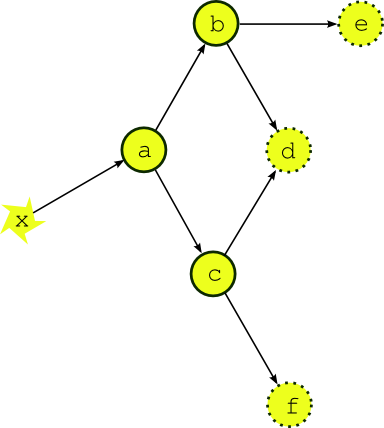
\includegraphics[width=6cm]{inkscape-svg/dep-one-cycle} 
    \end{center}
    \caption[Single cycle dependency graph for a simple suite]{\small
    The dependency graph for a single forecast cycle of a simple example
    suite. Tasks {\em a, b,} and {\em c} represent forecast models,
    {\em d, e} and {\em f} are post processing or product generation
    tasks, and {\em x} represents external data that the upstream
    forecast model depends on.}
    \label{fig-dep-one} 
\end{figure} 

\begin{figure}
    \begin{center}
        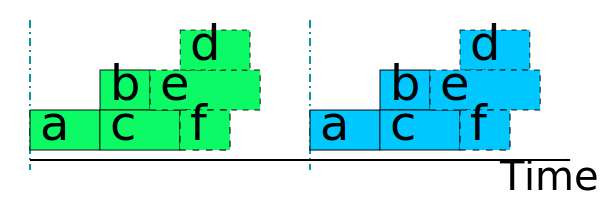
\includegraphics[width=8cm]{inkscape-svg/timeline-one}
    \end{center}
    \caption[Single cycle job schedules for real time operation]{\small
    The optimal job schedule for two consecutive cycles of our example
    suite during real time operation, assuming that all tasks trigger 
    off upstream tasks finishing completely. The horizontal extent of
    a task bar represents its execution time, and the vertical blue
    lines show when the external driving data becomes available.}
    \label{fig-time-one}
\end{figure}

Figure~\ref{fig-time-one} shows the optimal job schedule for two
consecutive cycles of the example suite in real time operation, given
execution times represented by the horizontal extent of the task bars.
There is a time gap between cycles as the suite waits on new external
driving data.  Each task in the example suite happens to trigger off
upstream tasks {\em finishing}, rather than off any intermediate output
or event; this is merely a simplification that makes for clearer diagrams.

\begin{figure}
    \begin{center}
        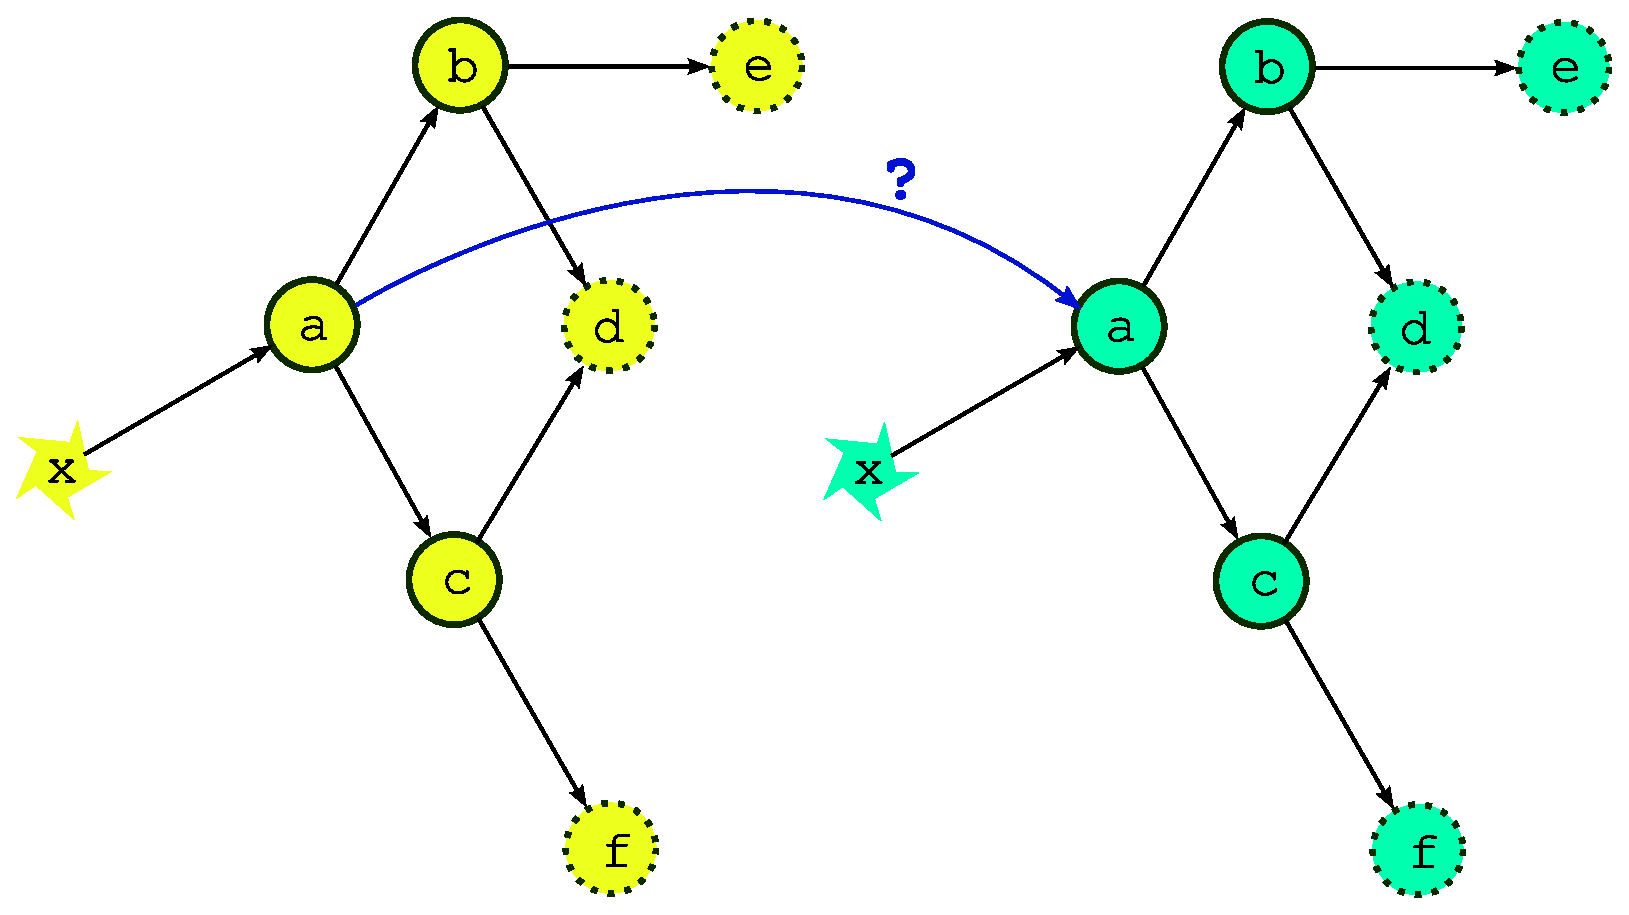
\includegraphics[width=10cm]{inkscape-svg/dep-two-cycles-linked} 
    \end{center}
    \caption[What if the external data is available early?]{\small If
    the external driving data is available in advance, can we start
    running the next cycle early?} 
    \label{fig-dep-two-linked}
\end{figure}

\begin{figure}
    \begin{center}
        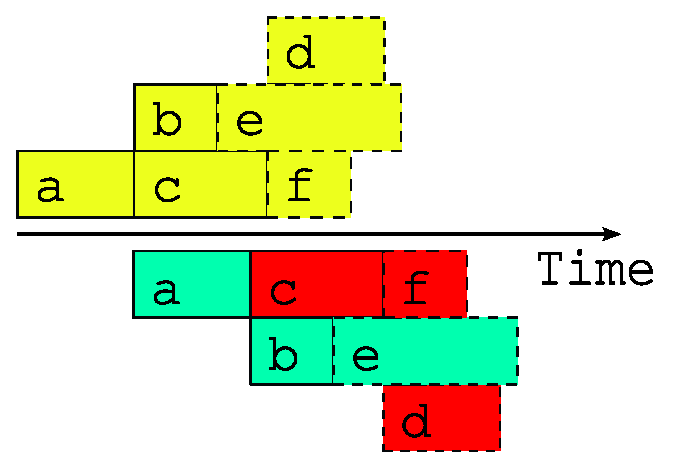
\includegraphics[width=6cm]{inkscape-svg/timeline-one-c} 
    \end{center}
    \caption[Attempted overlap of consective single-cycle job
    schedules]{\small A naive attempt to overlap two consecutive cycles
    using the single-cycle dependency graph. The red shaded tasks will
    fail because of dependency violations (or will not be able to run
    because of upstream dependency violations).} 
    \label{fig-overlap}
\end{figure} 

\begin{figure}
    \begin{center}
        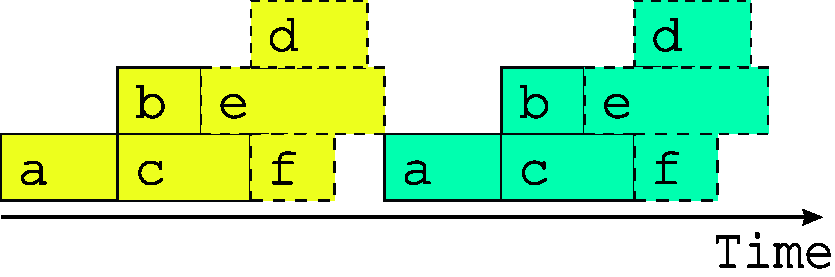
\includegraphics[width=8cm]{inkscape-svg/timeline-one-a} 
    \end{center}
    \caption[The only safe multicycle job schedule?]{\small The best that
    can be done {\em in general} when intercycle dependencies are
    ignored.} 
    \label{fig-job-no-overlap}
\end{figure} 

Now the question arises, what happens if the external driving data for
upcoming cycles is available in advance, as it would be after a
significant delay in operations, or when running a historical case
study?  The forecast model {\em a} depends only on the external data
and, implicitly at this stage of the discussion, on its own previous
instance for a model ``background state''. Thus, as alluded to in
Figure~\ref{fig-dep-two-linked}, task {\em a} could in principle start
immediately its predecessor has finished.  Figure~\ref{fig-overlap}
shows, however, that starting a whole new cycle at this point is
dangerous - it results in dependency violations in half of the tasks in
the simple example suite. In fact the situation is even worse than this
- what if task {\em b} in the first cycle is delayed for any reason {\em
after} the second cycle has been launched? Clearly we must consider
handling intercycle dependencies explicitly in order to solve this
problem, or else agree never to start the next cycle early, as
is illustrated in Figure~\ref{fig-job-no-overlap}.


\subsection{Intercycle Dependencies} 
\label{IntercycleDependencies}

In any non-trivial suite dependencies between tasks in different cycles
exist. Forecast models typically depend on their own most recent
previous forecast for an initial ``background state'', and different
types of tasks in different forecast cycles can also be linked (e.g.\
the complicated relationship between the weather and river models in
EcoConnect). In real time operation these intercycle dependencies
can be ignored because they are automatically satisfied when each cycle
necessarily finishes before the next one begins. This is just as well
because they dramatically increase the complexity of the dependency
graph of even the simplest suites, by destroying the clean boundary
between forecast cycles. Figure~\ref{fig-dep-multi} illustrates the
problem for our simple example suite assuming the minimal likely
intercycle dependence: the forecast models ($a$, $b$, and $c$) each
depend on their own previous instances.

For this reason, and because we tend to imagine that forecasting systems
always run in distinct cycles, existing schedulers (as far as the author
is aware!) ignore intercycle dependencies and therefore {\em require} a
series of distinct cycles at all times. While this does not affect
normal real time operation it can be a serious impediment when advance
availability of external driving data makes it possible, in principle,
to run some tasks from upcoming cycles before the current cycle is
finished - as suggested at the end of the previous section. This occurs
after delays (late arrival of external data, system maintenance, etc.)
and, to an even greater extent, in historical case studies, and parallel
test suites that are delayed with respect to the main operation. It is
a serious problem, in particular, for suites that have little downtime
between forecast cycles and therefore take many cycles to catch up
after a delay. Without taking account of intercycle dependencies, the
best that can be done, in general, is to reduce the gap between cycles
to zero as shown in Figure~\ref{fig-job-no-overlap}. A limited crude
overlap of the single cycle job schedule may be possible for specific
task sets but the allowable overlap may change if new tasks are added,
and it is still dangerous: it amounts to running different parts of a
dependant system as if they were not dependant and as such it cannot be
guaranteed that any unforeseen delay occuring in one cycle after the 
next has begun (e.g.\ due to resource contention or task failures) won't
result in dependency violations in the next.

\begin{figure}
    \begin{center}
        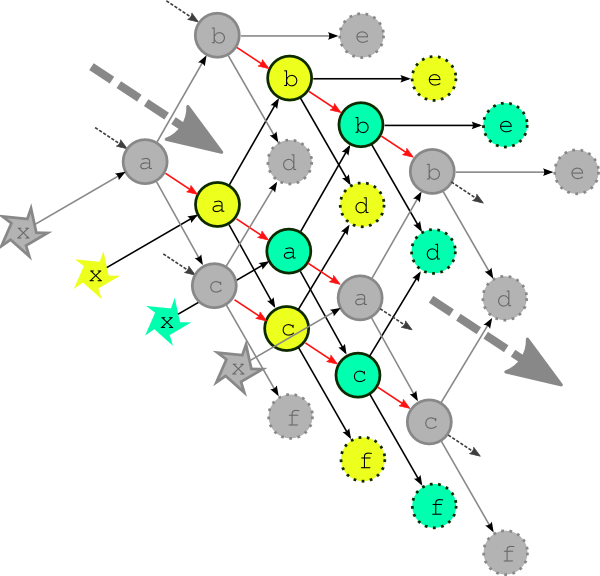
\includegraphics[width=8cm]{inkscape-svg/dep-multi-cycle} 
    \end{center}
    \caption[Complete multicycle dependency graph]{\small The complete
    dependency graph for the example suite, assuming the least possible
    intercycle dependence: the forecast models ($a$, $b$, and $c$)
    depend on their own previous instances. The dashed arrows show
    connections to previous and subsequent forecast cycles.} 
    \label{fig-dep-multi}
\end{figure}

\begin{figure}
    \begin{center}
        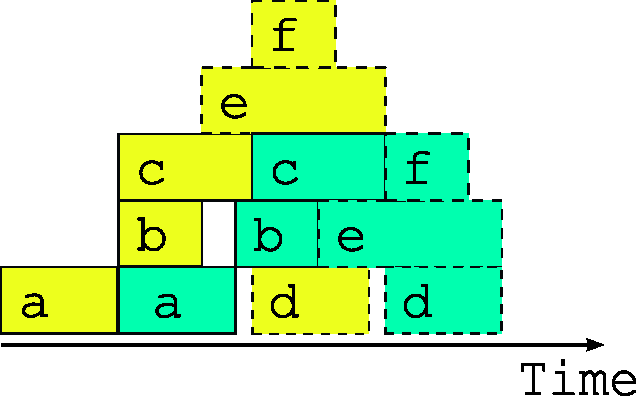
\includegraphics[width=6cm]{inkscape-svg/timeline-two-cycles-optimal} 
    \end{center}
    \caption[Optimal two-cycle job schedule]{\small Optimal two cycle
    job schedule when the next cycle's driving data is available in
    advance, possible in principle when intercycle dependencies are
    handled explicitly.} 
    \label{fig-optimal-two}
\end{figure} 

Figure~\ref{fig-optimal-two} shows, in contrast to
Figure~\ref{fig-overlap}, the optimal two cycle job schedule obtained by
respecting all intercycle dependencies. It must be noted, however, that
this job schedule assumes ideal conditions with no delays due to
resource contention or anything else - i.e.\ every task is able to run
in its alotted time as soon as it is ready to run. The scheduler running
this suite must be able to adapt dynamically to external conditions 
that impact on multicycle scheduling in the presence of
intercycle dependencies or else, again, risk bringing the system down
with dependency violations.

\begin{figure}
    \begin{center}
        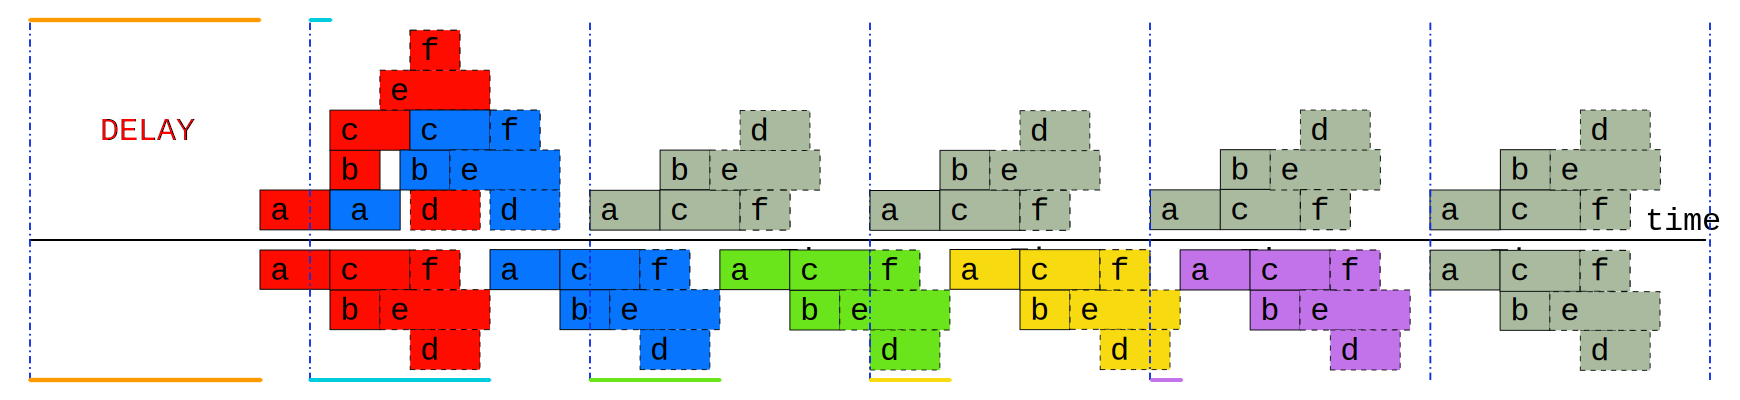
\includegraphics[width=12cm]{inkscape-svg/timeline-three} 
    \end{center}
    \caption[Post delay comparison of job schedules]{\small Job
    schedules for the example suite after a delay of almost one whole
    forecast cycle, when intercycle dependencies are
    taken into account (above the time axis), and when they are not
    (below the time axis). The colored lines indicate the time that
    each cycle is delayed, and normal ``caught up'' cycles
    are shaded gray.} 
    \label{fig-time-three}
\end{figure} 

\begin{figure}
    \begin{center} 
        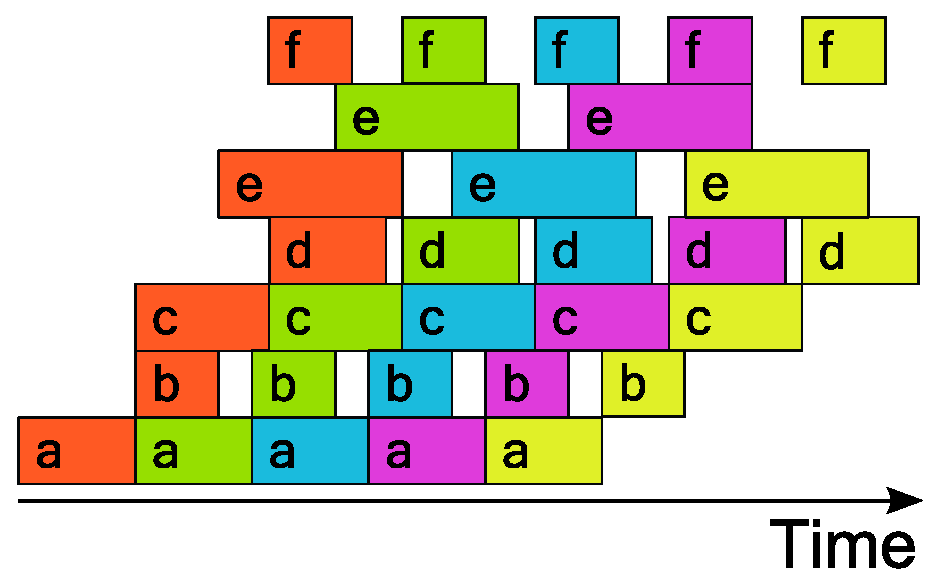
\includegraphics[width=8cm]{inkscape-svg/timeline-two}
    \end{center} 
    \caption[Optimal job schedule when all external data is
    available]{\small Job schedules for the example suite in case study
    mode, or after a long delay, when the external driving data are
    available many cycles in advance. Above the time axis is the optimal
    schedule obtained when the suite is constrained only by its true
    dependencies, as in Figure \ref{fig-dep-two-linked}, and underneath
    is the best that can be done, in general, when intercycle
    dependencies are ignored.} 
    \label{fig-time-two}
\end{figure} 

To further illustrate the potential benefits of proper intercycle
dependency handling, Figure~\ref{fig-time-three} shows an operational
delay of almost one whole cycle in a suite with little downtime between
cycles. Above the time axis is the optimal schedule that is possible, in
principle, when intercycle dependencies are taken into account, and
below is the only safe schedule possible {\em in general} when they are
ignored.  In the former case, even the cycle immediately after the delay
is hardly affected, and subsequent cycles are all on time, whilst in the
latter case it takes five full cycles to catch up to normal real time
operation.
%Note that simply overlapping the single cycle schedules of
%Figure~\ref{fig-time-one} from the same start point would have resulted
%in dependency violation by task {\em c}.

Similarly, Figure~\ref{fig-time-two} shows example suite job schedules
for an historical case study, or when catching up after a very long
delay; i.e.\ when the external driving data are available many cycles in
advance.  Task {\em a}, which as the most upstream forecast model is
likely to be a resource intensive atmosphere or ocean model, has no
upstream dependence on cotemporal tasks and can therefore run
continuously, regardless of how much downstream processing is yet to be
completed in its own, or any previous, forecast cycle (actually, task
{\em a} does depend on cotemporal task {\em x} which waits on the
external driving data, but that returns immediately when the external
data is available in advance, so the result stands). The other forecast
models can also cycle continuously or with short gap between, and some
post processing tasks, which have no previous-instance dependence, can
run continuously or even overlap (e.g.\ {\em e} in this case). Thus,
even for this very simple example suite, tasks from three or four
different cycles can in principle run simultaneously at any given time. 
In fact, if our tasks are able to trigger off internal outputs of 
upstream tasks, rather than waiting on full completion, successive
instances of the forecast models could overlap as well (because model
restart outputs are generally be completed early in the forecast) for an
even more efficient job schedule. 

Finally, we note again that a good job scheduler should be able to
dynamically adapt to delays in any part of the suite due to resource
contention, varying run times, or anything else that will inevitably
modify the depicted job schedules. 

\subsection{The Cylc Scheduling Algorithm} 
\label{TheCylcSchedulingAlgorithm}

\begin{figure}
    \begin{center} 
        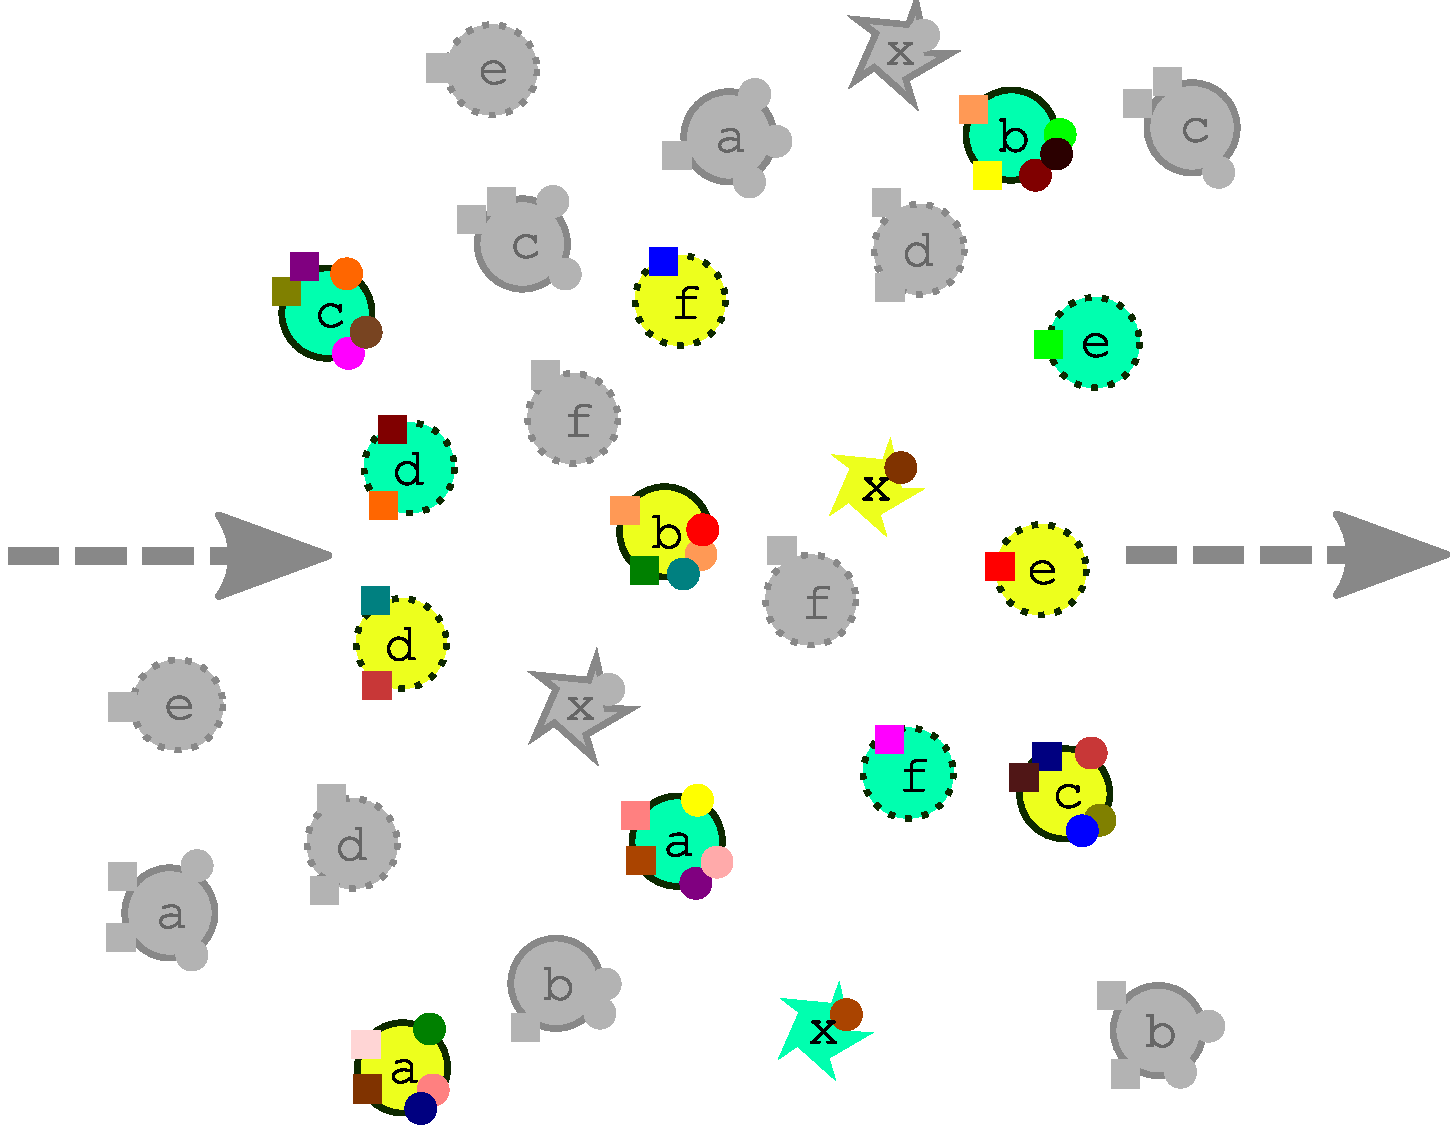
\includegraphics[width=8cm]{inkscape-svg/task-pool}
    \end{center} 
    \caption[The cylc task pool]{\small How cylc sees the task pool, in
    contrast to the full dependency diagram of Figure~\ref{fig-dep-multi}.} 
    \label{fig-task-pool}
\end{figure} 

This section explains how cylc achieves the optimal multicycle
scheduling described above. 

Cylc manages a pool of proxy objects that represent real tasks in the
forecasting system. A task proxy object can run the real task when its
prerequisites are satisfied, and can receive reports of completed
outputs from the real task as it runs. There is no global cycling
mechanism to advance the system in time; instead each individual task
proxy has a private cycle time and spawns its own successor at the right
time (which depends only on the task's own type and state). Task proxies
are self-contained and do not know what other tasks exist in the system,
they just know their own prerequisites and outputs.  Prerequisites can
equally represent intra- and intercycle dependencies, and the task pool
can be populated with tasks having many different cycles. Now,
whenever any task proxy changes state (as a result of an output
completion message, for example) cylc gets the entire pool to interact
indiscriminately, {\em regardless of cycle times}, in an attempt to
match unsatisfied prerequisites with completed outputs.\footnote{In fact
this dependency negotiation goes through a middleman or broker object,
which reduces the interaction scaling from $n^2$ to $n$, where $n$ is
the number of task proxies.} 

Thus without using global cycling mechanisms, and treating all
dependencies equally, cylc in effect gets a set of individual tasks to
self-organise by negotiating their own dependencies: optimal scheduling,
as illustrated in the previous section, emerges naturally at run time.

In addition, cylc makes no distinction between delayed and real time
operation. In delayed operation the tasks that gather the system's
external driving data will return immediately (because the data is
already available) and the system will only be constrained by its
internal dependencies. In real time operation, the data gathering tasks
will return only when the external data becomes available (normally at
some known time interval after the task's nominal cycle time), delaying
downstream tasks until then, by which time the previous forecast cycle
will have completed. A cylc suite thus transitions seamlessly from
optimal multicycle scheduling to ``normal'' distinct forecast cycles as
it catches up to real time operation.

Note that in addition to achieving optimal scheduling, this algorithm is
extremely simple. The operator does not have to construct a special
``suite'' in which order of execution or explicit dependency
relationships are specified (except implicitly, in that each task's
prerequisites must be matched by someone's outputs). Instead the entire
forecasting system is defined by a simple list of tasks each of which,
in effect, thinks it is alone in the world (even a standalone task must
know its own prerequisites and outputs).

%\footnote{However, you can still use explicit task dependence if you
%wish: just make a task depend on an explicitly named upstream supplier
%{\em finishing} rather than on the upstream output that is the actual
%prerequisite of interest. However, framing prerequisites in terms of
%required input filenames, or similar, results in a more flexible
%system: tasks can easily be ``hot replaced'' by others that generate
%similar outputs.}

Perhaps the most difficult problem encountered during cylc
implementation was how to arrange that every task proxy object exists by
the time it is needed, but not too much earlier, and does not die too
long after it is no longer needed. This engendered no small amount
of hair pulling and teeth gnashing, but once achieved the complexities
therein are entirely hidden from the user.

%In other words the task pool must include waiting tasks whose
%prerequisites may {\em soon} be satisfied (but preferably no waiting
%tasks whose prerequisites will not be satisfied for some time yet),
%tasks that are currently running, and finished tasks whose outputs
%could still be needed by any current or future waiting task (but
%preferably not any finished tasks whose output will no longer be needed
%by anyone). 



\pagebreak
\section{The Cylc Command Set}

Cylc commands are self-documenting. Section~\ref{CommandReference}
contains the complete {\em Command Reference}. 

\lstset{language=usage}
\lstinputlisting{command-usage/help.txt}

\pagebreak
\section{Installation And Testing} 
\label{InstallationAndTesting}

\subsection{Requirements} 
\label{Requirements}

\begin{itemize}
    \item Unix or Linux
    \item Python
    \item Pyro (Python Remote Objects)
\end{itemize}

Cylc has been tested with Python~2.6, and Pyro~3.9 and 3.10,
but it should work with any recent version of Python~2 and Pyro~3.

\subsection{Getting Cylc} 
\label{GettingCylc}

See Appendix~\ref{Pyro} for Pyro download directions.

Cylc is currently maintained using {\em darcs} (http://darcs.net), a
distributed revision control system. If you need to develop cylc you can
request a clone of the repository, otherwise you will receive a cylc
release tarball. 

\subsection{Installation} 
\label{Installation}

Pyro has its own installation instructions; it installs easily into the
standard Python modules path.

Cylc is designed to be installed into a normal user account: simply
unpack the tarball, or move the repository, to the location of your
choice (typically \lstinline=$HOME/cylc=). There is no ``build'' step
required.

\subsection{Environment} 
\label{Environment}

\lstset{language=bash} 

The cylc bin directory must be in your executable search path and the
cylc source directories must be in your Python module search path. To
configure your current command shell for cylc, source the environment
script \lstinline=cylc-env.sh= from the directory it resides in (i.e.\
the top level of your cylc installation):

\begin{lstlisting}
$ cd $HOME/cylc            # (the install location)
$ . cylc-env.sh
\end{lstlisting}

Or put the following in your (sh-style) login script:

\begin{lstlisting}
# CYLC
export CYLC_DIR=$HOME/cylc  # (the install location)
. $CYLC_DIR/cylc-env.sh
\end{lstlisting}


\subsection{Testing} 
\label{Testing}

You can test the new installation by running the packaged ``userguide''
example suite (which implements the simple six-task suite used to 
illustrate the first section of the userguide). The example suite
should work ``out of the box'' in real and dummy mode, using the simple
sequence of commands presented in the Quick Start Guide. 
For more information on the various example suites that come with cylc
refer to {\em A Complete Working Example}
(Section~\ref{ACompleteWorkingExample}), and {\em Other Working
Examples} (Section~\ref{OtherWorkingExamples}).  

\pagebreak
\section{Quick Start Guide} 
\label{QuickStartGuide}

\lstset{language=bash}

This section is intended as a quick introduction to, or reminder of,
basic cylc functionality. The specific command line listings below use
the packaged cylc ``userguide'' example suite. Refer to 
\lstinline=cylc help=, the {\em Command Reference}
(Section~\ref{CommandReference}), and
upcoming sections of this document for more detailed information on
available commands, options, and operations.  {\em A Complete Working
Example} (Section~\ref{ACompleteWorkingExample}) describes the
userguide example suite in detail.

\subsection{Starting A Pyro Nameserver}
\label{QuickStartingAPyroNameserver}

Pyro (Appendix~\ref{Pyro}) is the object oriented Python RPC framework
that allows suite tasks to communicate with their proxy objects inside
a cylc scheduler. First check to see if there is already a Pyro
nameserver (\lstinline=pyro-ns=) running on your network segment:

\begin{lstlisting}
# search for a Pyro nameserver on the network
$ pyro-nsc ping
Locator: searching Pyro Name Server...
Locator: retry 1
Locator: searching Pyro Name Server...
Locator: retry 1
Trying host oliverh-33191VL
Locator: contacting Pyro Name Server...
NS is at 127.0.0.2 (oliverh-33191VL.greta.niwa.co.nz) port 9090
NS is up and running!

# search for a Pyro nameserver on a specific host
$ pyro-nsc -h localhost ping
Locator: contacting Pyro Name Server...
NS is at 127.0.0.1 (localhost) port 9090
NS is up and running!
\end{lstlisting}

If not, start one up as follows:

\begin{lstlisting}
# start a Pyro nameserver
$ pyro-ns
*** Pyro Name Server ***
Name server listening on: ('0.0.0.0', 9090)
Broadcast server listening on: ('255.255.255.255', 9090)
URI is: PYRO://192.168.56.146:9090/c0a838921e021d8a88b563c085c323e5f4
URI written to: /home/oliverh/Pyro_NS_URI
Name Server started.
\end{lstlisting}

The Pyro nameserver is unfortunately not a daemon process, because it
also has to run on platforms such as Microsoft Windows, but you can
start it with the \lstinline=nohup= command 
(see \lstinline=man nohup=) to effectively detach it from your terminal
login session.

\subsection{Starting The Cylc Lockserver}
\label{QuickStartingTheCylcLockserver}

The cylc lockserver prevents you from accidentally running multiple
instances of the same suite or task (at the same cycle time) at once,
which could result in a corrupted system state (your real forcasting
system, that is, not cylc) or other problems. 

It consists of a {\em Unix daemon} 
\lstinline=$CYLC_DIR/admin/cylclockd= that runs autonomously, brokering
locks for all cylc suites running on the network, and a command line
user interface, \lstinline=cylc lockserver=

The daemon should be started at boot time as a special system user, but
for testing purposes you can run it as a normal user as follows: 
Edit \lstinline=$CYLC_DIR/admin/cylclockd.conf.test= to set process ID,
log, and state file locations, then start it up like this:

\begin{lstlisting}
cylclockd -f cylclockd.conf.test start
\end{lstlisting}

See \lstinline=cylclockd --help= for other usage information.

Alternatively, you can choose not to use the lockserver for the moment:

\begin{lstlisting}
cylc preferences --use-lockserver=N
\end{lstlisting}


\subsection{Defining A Suite} 
\label{QuickDefiningASuite}

A cylc suite is defined by a set of simple {\em task definition files}
that describe the properties of each task that are relevant from a
scheduling perspective (see {\em Suite Definition},
Section~\ref{SuiteDefinition}); in particular, for cylc, the
prerequisites and outputs of each task.

In addition, a few cylc commands must be inserted into the scripts that
execute the suite tasks, or otherwise you can use cylc's {\em task
wrapping} mechanism (Section~\ref{TaskWrapping}) to run existing scripts
unmodified.

The complete suite definition and implementation for the ``userguide
example suite'' is provided in \lstinline=$CYLC_DIR/suites/userguide=. 

\subsection{Suite Registration}
\label{QuickSuiteRegistration}

\begin{lstlisting}
cylc register $CYLC_DIR/suites/userguide userguide 
\end{lstlisting}

This associates a suite definition directory with a {\em suite name}
that will henceforth be used to target the suite via cylc commands. 
\lstinline=cylc register --list= shows your suite registrations.

\subsection{Starting The Suite}
\label{QuickStartingTheSuite}

\begin{lstlisting}
cylc start userguide 2009082312
\end{lstlisting}

%See {\em Running Cylc Suites}, Section~\ref{RunningCylcSuites}.

In real mode operation (as opposed to {\em dummy mode},
Section~\ref{DummyMode}) {\em do not choose an initial cycle time in the
future} or nothing will happen until that time arrives!

You can run multiple instances of the userguide example suite at once,
under different names; the suite name is used in all I/O file paths so
the different instances will not interfere. 

\subsection{Following Suite Progress}
\label{QuickFollowingSuiteProgress}

\begin{figure}
    \begin{center}
        %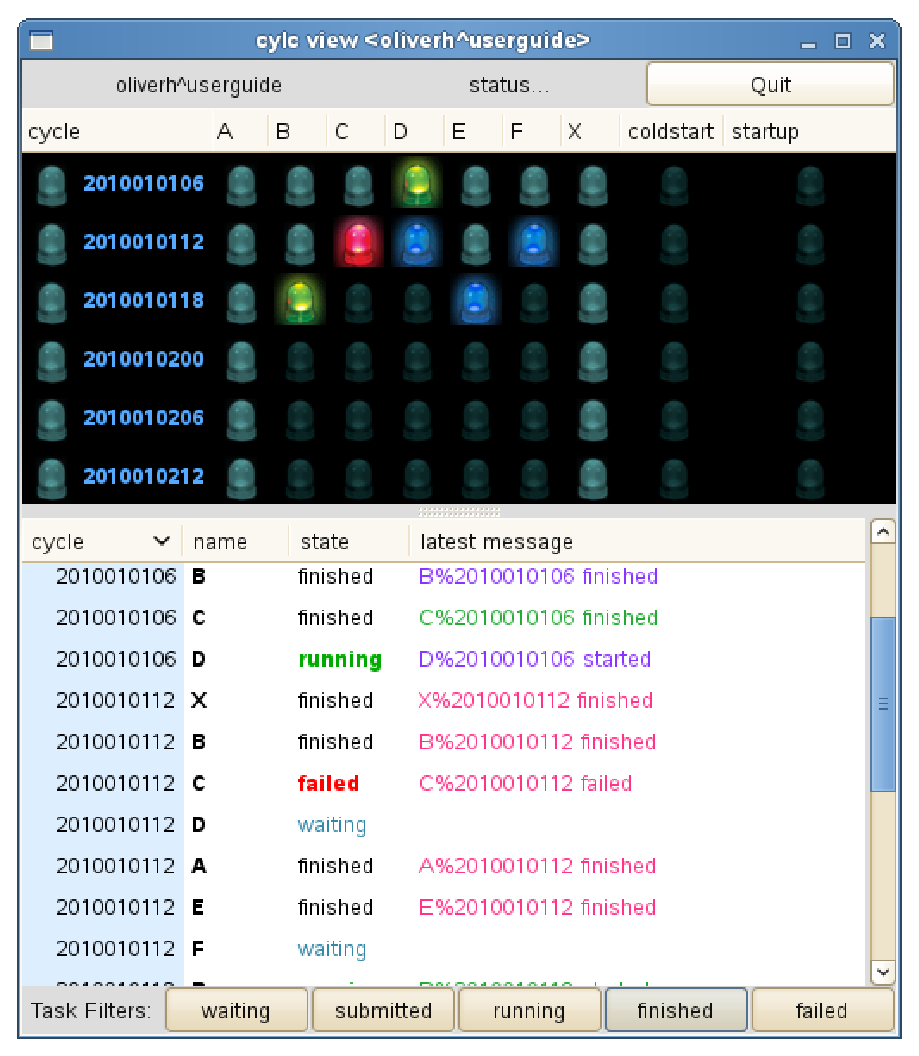
\includegraphics[width=12cm]{monitor} 
        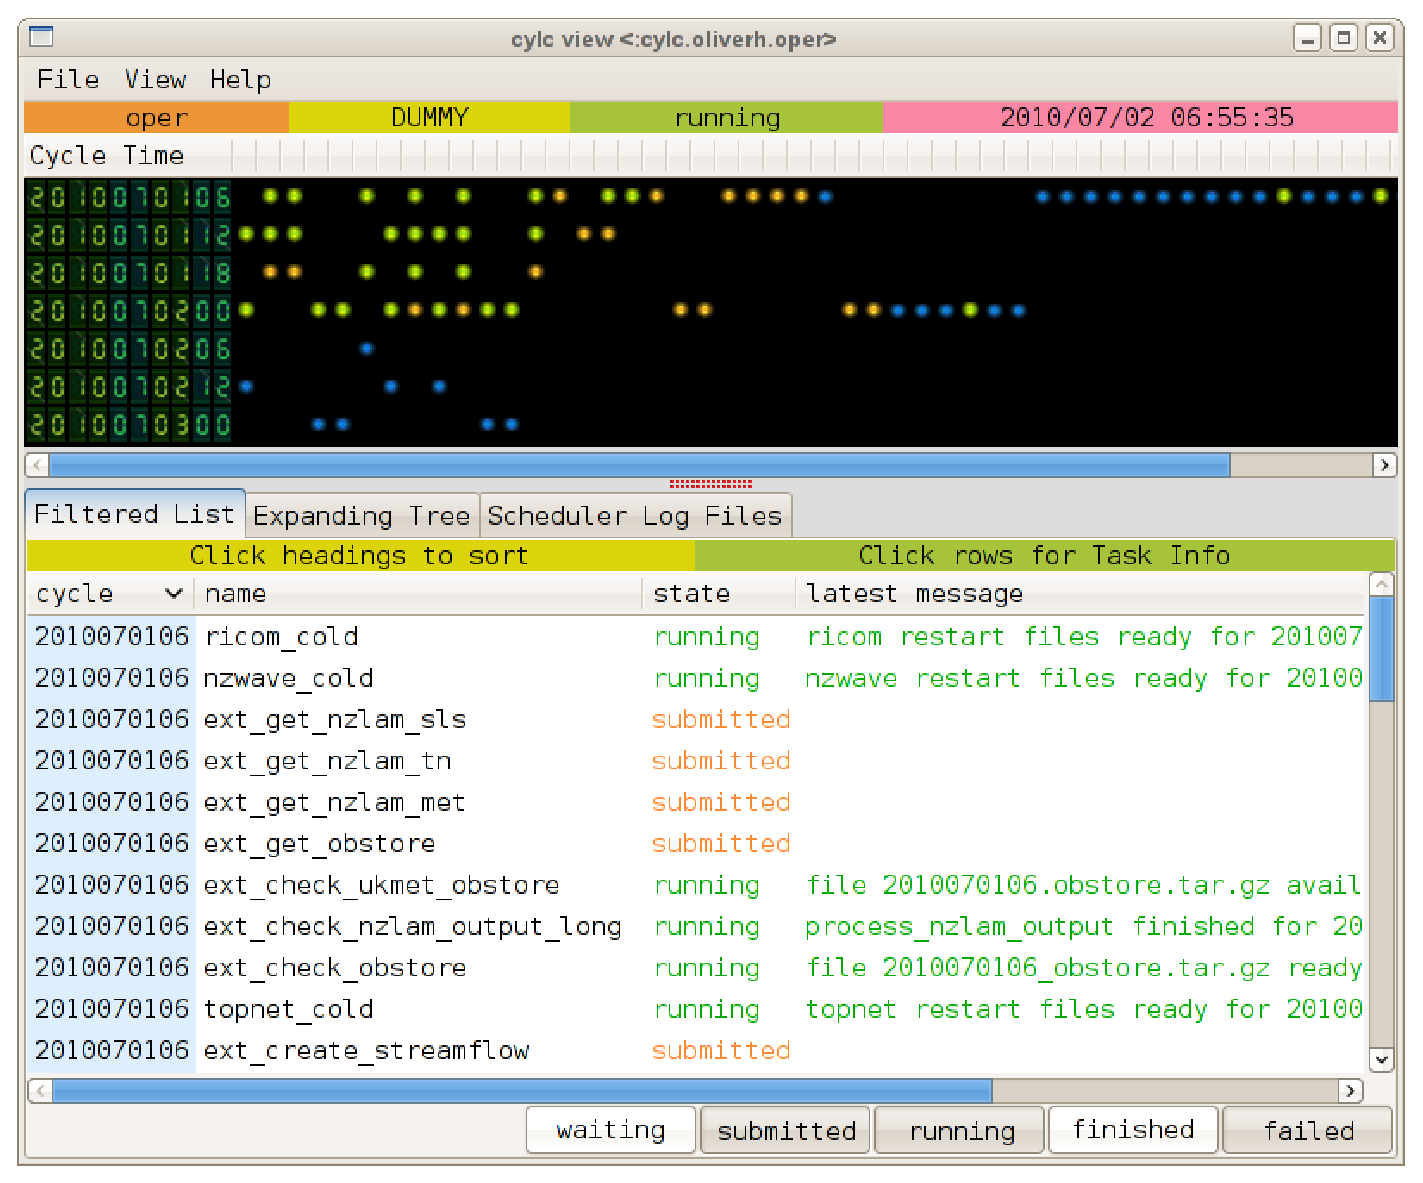
\includegraphics[width=12cm]{cylc-view-ecoconnect} 
    \end{center}
    \caption{\small {\em cylc view} screenshot}
    \label{fig-monitor} 
\end{figure} 

{\em cylc view} provides real time access to a lot of information as 
the suite evolves, most of which can also be accessed via the
commandline interface (\lstinline=cylc ping, show=, etc.).

\begin{lstlisting}
cylc view userguide &
\end{lstlisting}

Cylc {\em Log Files} (Section~\ref{SuiteLogFiles}) are located 
under \lstinline=$HOME/.cylc/logging/SUITE= (you can use
\lstinline=cylc preferences= to change the default location). Each task
has its own log file for task-specific events and the \lstinline=main=
log file records all events in sequence.

You can also retrieve information from running cylc suites with the 
\lstinline=cylc show= command:

\lstset{language=}
\begin{lstlisting}
% cylc show userguide X%2010010112
_______________________________
Task X%2010010112 in userguide:
 + => prerequisite satisfied, or output completed
 - => prerequisite NOT satisfied, or output NOT completed
______________
Prerequisites:
(None)
________
Outputs:
 + X%2010010112 completed
 + X%2010010112 finished
 + X%2010010112 started
 + obs data ready for 2010010112
______
Other:
delayed start time reached ... True
\end{lstlisting}

\lstset{language=bash}
\subsection{Shutdown And Restart}
\label{QuickShutdownAndRestart}

\lstset{language=bash}

Before shutting a suite down - or indeed using any of the other cylc
commands that can change the state of a running suite but are not 
covered in this Quick Start Guide (reset, kill, purge, pause, etc.) -
you need to {\em unlock} the suite:

\begin{lstlisting}
cylc unlock userguide
cylc stop userguide
\end{lstlisting}

You can restart a suite from its most recent previous state:

\begin{lstlisting}
cylc restart userguide
\end{lstlisting}
or from the state recorded in a particular named state dump file 
(cylc automatically dumps extra time-stamped state files prior to any
suite intervention so that you can easily revert to the
pre-intervention state in case of disaster). See {\em Restarts}
(Section~\ref{Restarts}) for more information.

\pagebreak
\section{Suite Definition} 
\label{SuiteDefinition}

%Cylc sees a forecasting system as an evolving, self-organising pool of
%tasks with clearly defined {\em prerequisites} and {\em outputs}, as
%explained in {\em The Cylc Scheduling Algorithm} (Section~\ref{TheCylcSchedulingAlgorithm}). 

Your suite must be divided into tasks with clearly defined
prerequisites and outputs (Section~\ref{TaskPrerequisitesAndOutputs}). Then
the properties of each task that are relevant to scheduling must be
declared in {\em Task Definition Files}
(Section~\ref{TaskDefinitionFiles}). One such property is the script or
executable that should be called to run the real task when
it is ready to run. These {\em Task Scripts} (Section~\ref{TaskScripts})
can be located anywhere, but if you are creating a new suite you may
wish to keep them in a central location along with the suite task
definition files.  The packaged cylc example suites reside under
\lstinline=$CYLC_DIR/suites=, for
example:

\lstset{language=bash}

\begin{lstlisting}
# suite userguide:
$CYLC_DIR/suites/userguide/

   taskdef/            # TASK DEFINITION FILES, e.g.:
      A.def              # defines task A
      B.def              # defines task B
      #...

   scripts/            # TASK SCRIPTS (automatically added to PATH)
      A.sh               # e.g. called by cylc to execute task A
      B.sh               # e.g. called by cylc to execute task B
      #...

   suite.rc            # AUTOGENERATED ONCE (customizable)

   configured/         # AUTOGENERATED suite-specific python modules
      class_A.py
      class_B.py
      #...
      task_classes.py
      task_list.py
\end{lstlisting}

External suites should be maintained elsewhere in their own version
control repositories, with tags to indicate compatibility with
particular versions of cylc.

\subsection{Granularity} 
\label{Granularity}

A suite can contain a small number of large, internally complex tasks;
a large number of small, simple tasks; or anything in between. However,
cylc can easily handle large task numbers, and is entirely self
organising, so there are advantages fine-graining a suite:

\begin{itemize}
    \item a more modular and transparent suite.

    \item better functional parallelism: multiple processes running
        at the same time.

    \item faster failure recovery: rerun just the tasks(s) that failed. 

    \item the same external task script (e.g.\ for moving files around)
        can often be invoked, with different arguments, for multiple
        tasks.

\end{itemize}





\subsection{Suite Task Guidelines} 
\label{SuiteTaskGuidelines}

The first three the following subsections are meant to encourage good
suite design in general, and the final two are more cylc-specific.

\subsubsection{Restartability}

It should be possible to restart a failed task (after fixing the
problem) by simply resubmitting it for the same cycle time. In other
words, failure at any point during task execution should not render a
restart impossible by corrupting the state of some internal-use files,
or similar. 

\subsubsection{Previous Instance Dependence} 

A task that in principle does not depend on a previous instance of
itself (i.e.\ on the same task at a previous cycle time) should be able
to run as soon as its prerequisites are satisfied, even if one or more
of its predecessors has not finished (or even started) yet.  Post
processing tasks are typically of this type - they should be able to run
as soon as the files they process exist, regardless of whether or not
the processing of files from any previous cycles has occurred yet.

Similarly, a warm-cycled forecast model, which depends on a previous
instance via its restart prerequisites, should be able to run as soon as
its prerequisites (including the restart ones) are satisfied.

If this is not the case in practice, perhaps because of the task in
question makes use of a temporary workspace that is not labelled by
cycle time, then cylc's sequential task type modifier see {\em Task
Types} (Section~\ref{TaskTypes}) can easily force sequential execution
of particular tasks, but the resulting suite will be somewhat less
efficient than it could be.

\subsubsection{Multicycle Restartability} 

A warm-cycled forecast model's restart files, which are written in
one cycle and read in the next, should not simply be overwritten with
each new run. Otherwise these files could be corrupted if the task is
accidentally invoked at the wrong cycle time, thereby breaking the task
for the correct cycle (and a cold start will subsequently be required).
Instead, consider organising restart files by cycle time, through a file
or directory naming convention, and keep them in a simple cycle-time
based rolling archive. Then (given all other cycle time dependent
inputs) the task can easily be rerun for any cycle still in the archive.

\subsubsection{Reporting Outputs and Failures}

All outputs that other tasks may depend on must be reported via cylc's
simple messaging interface, which is explained in {\em Prerequisites and
Outputs} (Section~\ref{TaskPrerequisitesAndOutputs}). Similarly, fatal
errors must be reported by the same mechanism, otherwise cylc will think
the failed task is still running. 

Ideally, important errors should be checked for explicitly, and lesser
fatal errors (e.g.\ failure to create an output directory) can be
trapped by the shell and handled with an automatic message. The
userguide example task script listings of
Section~\ref{ACompleteWorkingExample} show how to do this.

\subsubsection{Contact Tasks Must Wait On Data}

Most tasks in a cylc suite know their own cycle time, but they don't
know or care what the wall clock time is.  They just run when their
prerequisites are satisfied, i.e.\  when other tasks say their input
files (usually) are ready for use. The only connection between cylc
suites and the real world are the {\em contact tasks} (see {\em Task
Types}, Section~\ref{TaskTypes} for more on this) which in addition to
their other prerequisites, if any, wait on a particular wall clock time
relative to their cycle time before running.  For example, a weather
model that assimilates real time observations should have an associated
contact task whose job is to report when those observations are ready
for use.  If in real time operation at nominal analysis time T, the obs
are expected at, say, T+3 hours, then the contact task should be
configured to launch at 3 hours past its cycle time (again, at the
earliest because its other prerequisites must also be satisfied).
If the suite is delayed by more than three hours, so that T+3 hours 
has already passed, then the contact task will launch immediately.
If there's any chance that the obs could in fact be ready at T+2 hours,
then the contact delay interval should be changed to 2 hours.  To allow
for possible late arrival of obs, which likely will happen on occasion,
the real contact task should have a wait loop in it: once running it
should check for the existence of the expected data immediately. If the
data isn't there the task must keep checking until it shows up, and only then
report its output completed to cylc. 


\subsection{Incremental Suite Construction} 
\label{IncrementalSuiteConstruction}

You can get the {\em scheduling} of a complex suite right without ever
having to run the real tasks, by testing incrementally in cylc's {\em
Dummy Mode} (Section~\ref{DummyMode}) as you define each task. Then (or
in parallel with the task definition process) you can also test the real
suite incrementally as you write its task scripts (by which cylc runs
the real tasks) by turning off all the tasks that you're not yet
interested in (this can be done through the \lstinline=--include= and
\lstinline=--exclude= scheduler options, or by commenting task names out
of the autogenerated task list.

Start by defining tasks at the top of the single-cycle dependency graph,
and testing in dummy mode each time a new task is added. This checks
that prerequisites and outputs match correctly. When the whole suite is
defined, begin writing the real task scripts in the same order, and test
in real mode with the as yet unimplemented tasks turned off (comment
them out of \lstinline=configured/task_list.py= or use the cylc
command line options provided for this purpose). 


\subsection{Task Prerequisites And Outputs}
\label{TaskPrerequisitesAndOutputs}

Cylc's scheduling algorithm matches one task's completed outputs with
another's unsatisfied prerequisites
(Section~\ref{TheCylcSchedulingAlgorithm}).  

Each task definition file must specify a list of prerequisites that have
to be satisfied before the task can run, and a list of outputs that will
be completed as the task runs. {\em These are just literal text
strings - messages that running tasks must send to their proxy objects,
inside the cylc scheduler, whenever they complete a registered output}.

In earlier versions of cylc an estimated run time for the task, and an
estimated completion time for each task output, had to be supplied in
the task definition, allowing very accurate simulation of each task
in cylc's dummy mode.  However, this added some complexity to the task
definition process, and because of inevitable variation in real task
effective run times due to resource contention it probably gives no
great benefit over the current simpler scheme: all dummy tasks are
assigned the same run time and their outputs reported in regular
intervals over that time - this is still a complete test of suite
meta-scheduling (i.e.\ tasks triggering as soon as their dependencies
are satisfied). 

\begin{itemize}
    \item A task proxy considers a registered output ``completed''
        if it has received a matching message from its external task.

    \item A task proxy considers a registered prerequisite ``satisfied''
        if another task proxy reports that it has a matching completed
        output.

\end{itemize}

A task with no prerequisites can start running immediately (i.e.\ as soon
as the proxy object is created) {\em unless} it is a ``contact task''
(below), which must also wait on a wall clock time relative to its cycle time.

{\em Every suite must contain at least one task with no prerequisites
to get things up and running}. These will normally be special oneoff
startup tasks (e.g.\ to clean out a full-suite workspace) and contact
tasks that wait on external input for each cycle.


\lstset{language=cylctaskdef} 

\subsubsection{Cycle Time}

{\em Prerequisites and outputs should always contain a cycle time} to
distinguish between different instances of a task (at different 
forecast cycles) that may coexist in the task pool at any time. 

Prerequisites that reflect same-cycle dependencies, which is the usual
case, should mention the host task's own cycle time, expressed as
\lstinline=$(CYCLE_TIME)= in task definition files.

For intercycle dependencies, the cycle time in a prerequisite message
should be expressed as some offset from the task's own cycle time, e.g.\
\lstinline=$(CYCLE_TIME - 6)=. However, the only intercycle dependencies
you are likely to encounter (see the TopNet model in EcoConnect,
Section~\ref{EcoConnect}, for a counter example) are the restart
dependencies of your warm cycled forecast models, and the prerequisites
and outputs for these are now registered automatically by cylc.

\subsubsection{Message Form}

The exact form of the messages does not matter so long as the
prerequisites match their corresponding and outputs. For example, if
the message, 
\begin{lstlisting}
"storm surge forecast fields ready for $(CYCLE_TIME)"
\end{lstlisting} 
is registered as an output by the task that generates said forecast
fields, then the exact same message should be registered as a
prerequisite by any task that requires that data as input
(presumably storm surge postprocessing tasks in this case). 

\subsubsection{Message Content}

Prerequisites and outputs typically refer to the completion of a file or
a group of files, but it can be any event that a task could conceivably
trigger off: database interactions, download of data from a network,
copying or archiving of files, etc.

For single file outputs the cylc message could include the actual
filename:
\begin{lstlisting}
"file surface-pressure-$(CYCLE_TIME).nc ready for use"
\end{lstlisting}
but there is no need to do this (see {\em Message Truth} below); you
might as well adopt a message format that applies equally well to
more general events and multi-file outputs:
\begin{lstlisting}
"surface pressure fields ready for $(CYCLE_TIME)"
\end{lstlisting}


\subsubsection{Message Truth}

{\em Cylc does not check that incoming messages are true.}  For example,
if the message refers to completion of a particular output file, cylc
does not check that the file actually exists as the reporting task
claims it does. There are two reasons for this: (1) cylc does not place
any restriction on the kind of event that can be used as a task trigger,
so it would be next to impossible for it to verify outputs in general,
and (2) there is actually no need for cylc to check because the tasks
themselves must necessarily do it, and they must immediately report
problems back to cylc before aborting (or in the worst case, neglect to
check and then fail for lack of required inputs, with the same result).


\subsubsection{Uniqueness}

Prerequisites need not be unique; i.e.\ multiple tasks can trigger off
the same event.

Outputs should probably be unique; otherwise a task that depends on a
particular output will trigger off the first task to provide it.


\subsection{Task Types} 
\label{TaskTypes}

In cylc, every task (sans cycle time, which is a task type parameter) is
a member of its own class, defined by python modules generated on
parsing the suite taskdef files (see \lstinline=cylc configure=).
Each task, via the taskdef \lstinline=TYPE= key, must declare itself to
be derived from one of two base classes that define its main properties:

\begin{itemize} 
    
    \item A \lstinline=free= task does not depend on outputs generated
        by a previous instance of its own class, which means successive
        instances of it can run in parallel if the opportunity arises
        (i.e.\ prerequisites allowing).  To allow this to happen, a free
        task spawns a successor as soon as it enters the {\em running}
        state\footnote{Spawning any earlier than this would bring no
        advantage, in terms of parallel execution, at the cost of
        unrestrained task breeding.}. Most non-forecast model tasks (pre
        and post processing tasks, etc.) should be of this type.

    \item A \lstinline=tied= task {\em does} depend on outputs generated
        by a previous instance of its own class. These are typically
        warm cycled forecast models which depend on ``restart'' files
        generated by the previous forecast, e.g.\ ``model background''
        data used in part to initialise the new forecast.
        Other prerequisites allowing, cylc can run successive forecast
        models as soon their restart files are available {\em if}
        those restart outputs are reported as soon as they are
        generated. However, successive instances of a forecast model will
        often run in sequence at best because of resource limitations,
        or because the model executable has not been modified to report
        mid-run outputs back to cylc at the time they occur (in which
        case all restart outputs will be reported complete at once when
        the model run finishes).

%    # *(2) A FORECAST_MODEL depends on a previous instance of the same
%    # task to provide special `restart' prerequisites: during a
%%    # forecast, a warm-cycling model will write out a state dump valid
%    # at the start time of the next forecast, for use in initialising
%    # it. Multiple restart outputs may be generated to allow one or more
%    # subsequent forecasts to be omitted if necessary. A forecast_model
%    # registers how many of these are generated, which cylc assumes are
%    # intended for use by the next N valid start times for the task and
%    # automatically adds special outputs and prerequisites to represent
%    # them in the suite. 
%    # A forecast model cannot start running until
%    # its restart prerequisite is satisfied, but the same prerequisite
%    # can potentially be satisfied by a restart output from any of the
%    # previous N forecasts. This allows cylc to continue running when
%    # one or more cycles of a particular model have to be omitted
%    # because of problems. But in normal operation we only want a model
%    # to trigger off the most recent previous forecast, which means that
%    # a forecast model cannot spawn a successor until its *last* restart
%    # output is completed (otherwise there is a chance the next-plus-one
%    # instance could come into existence and trigger before the the
%    # current instance, and so on, in normal operation). 
 
\end{itemize}


\subsubsection{Task Type Modifiers} 

A task may also declare one or more {\em modifiers}, after the main
type, that alter its behaviour to some extent:

\begin{itemize}
    \item A \lstinline=oneoff= task never spawns a successor; once it
        has finished and is no longer needed it will be removed from the
        system. This can be used for tasks that clean out a suite 
        workspace, for example, and {\em cold start} tasks that supply
        initial restart inputs to warm cycled forecast models. See also
        the \lstinline=COLDSTART_PREREQUISITES= task definition key, below.

    \item A \lstinline=sequential= task does not spawn a successor until it is
        finished. You can use this to force successive instances of a
        free or tied task to run in sequence if multiple instances of
        the real external task cannot be allowed to run at the same
        time (perhaps because they would interfere with each other
        through use of the same temporary files, or similar).

    \item A \lstinline=contact= task waits on an external event, such as
        incoming external data, i.e.\ it ``makes contact'' with the
        external world.  The event is expected at some defined time
        interval after the task cycle time (e.g.\ observational data
        might come 3.5 hours after its nominal validity time); see
        \lstinline=CONTACT_DELAY= below. In real time operation a contact task will
        not begin running until the clock time has reached this delayed
        start time. In catchup operation a contact task will begin
        running immediately (other prerequisites allowing) because the
        delayed start time has already passed.  
        

    % TO DO: PUT IN AN ``ADVANCED'' SECTION
    %\item A \lstinline=catchup_contact= task maintains awareness,
    %    through a class variable (i.e.\ not per instance), of whether or
    %    not it has `caught up' yet.  This can be used for rare occasions
    %    when some dependant task needs to behave differently according
    %    to whether its upstream contact task has caught up or not (in
    %    EcoConnect, only the TopNet river model).

    \item A \lstinline=dummy= task always invokes the cylc dummy task
        program, even when operating in real mode.  The dummy task
        program masquerades as the task it represents by reporting its
        registered outputs completed after a short interval. This can be
        used to ``fake'' provision of initial restart prerequisites to a
        forecast model whose real initial inputs have been put in place
        by some external means (perhaps a long ``spin up'' process)
        prior to starting the whole suite.

\end{itemize}



\subsection{Automatic Started And Finished Outputs}

Special {\em started} and {\em finished} outputs are automatically
registered for every task: 

\begin{lstlisting}
"foo%$(CYCLE_TIME) started"
"foo%$(CYCLE_TIME) finished"
\end{lstlisting}

Be aware that triggering off these messages introduces explicit
dependence on specific tasks, rather than on outputs that could be
provided, in principle, by any task, so this makes the suite somewhat
less flexible.


\subsection{Failure Messages}

\lstinline=cylc task-failed= should be used to report critical task
failures. A failed task will remain in the system until explicitly dealt
with by the operator.

\subsection{Completion Messages}

A special {\em task completed} message is sent whenever a tasks reports
success {\em or} failure:
\begin{lstlisting}
"foo completed for $(CYCLE_TIME)"
\end{lstlisting}
 
This can be useful if you want to trigger off an upstream task whether
or not it succeeded (e.g.: a data assimilation program that triggers
when a handful of separate obs processing programs have finished or
failed, where failure occurs if no obs of a particular type happen to be
available for the forecast cycle in question).


\subsection{Forecast Model Restart Outputs}

Task of the {\em tied} type (i.e.\ warm-cycled forecast models) must
declare, in their task definition files, the number of restart outputs
that they generate to satisfy the previous-instance dependence of their
successors. Cylc uses this information to automatically register special
restart outputs and prerequisites for the task. For example, if a
forecast model task called {\em foo} has a 6 hour cycle and generates
restart files for the next 2 cycles, the following prerequisite:

\begin{lstlisting}
"foo restart files ready for $(CYCLE_TIME)"
\end{lstlisting}

and the following two outputs:

\begin{lstlisting}
"foo restart files ready for $(CYCLE_TIME + 6)"
"foo restart files ready for $(CYCLE_TIME + 12)"
\end{lstlisting}

will be automatically registered for the task.

%\lstinline=cylc task-message= also has special options for reporting
%restart outputs so that you do not have to worry about typos in the
%message. 

\subsubsection{Restart Prerequisites at Suite Startup}

Note that while cylc automates registration of restart prerequisites and 
outputs for convenience, these are still nothing more than ordinary cylc
output messages, and there is one situation in which you still need to
register them explicitly in the taskdef file: {\em oneoff cold start
tasks} that provide the initial restart inputs to {\em other} tasks.
The userguide example suite shows this clearly.

% TO DO:
%    a task that behaves differently at different times should be 
%        handled using conditional prerequisites and outputs. For
%        example, a forecast model that does a long forecast at 06 and
%        18Z and a short forecast at other times. An alternative approach
%        though would be to split the task into two separate tasks that 
%        run in different cycles. If you want to do it this way then one
%        task will be providing restart outputs for the other, and vice
%        versa, which can be achieved by manually registering the same
%        restart output messages in the two tasks. 


\subsubsection{Use Of Tied Tasks Is Optional}

Tied tasks are merely a convenience to the suite designer in that they
automatically register the prerequisites and outputs that determine
forecast model intercycle restart dependencies. However, these automatic
prerequisites and outputs are just normal cylc messages; you could
easily use all {\em free} tasks and explicitly define the restart
prerequisites and outputs for your forecast models.

Alternatively, you could declare your forecast models to be
\lstinline=%TYPE free, sequential=.  Sequential tasks cannot start until
their previous instances have finished, so any restart prerequisites
will be implicitly satisfied. However, use of either the tied task type
or explicit restart dependencies does have the following advantages:

\begin{itemize}

    \item a more efficient system: forecast models can start up before
        their previous instances have finished, other prerequisites
        allowing.  
    
    \item automatic post-intervention recovery from nasty 
        failures, because cylc will know about the actual restart
        dependencies of your real tasks. For example, in the userguide
        example suite, if the weather model (task A) fails requiring a
        cold start 12 hours later, insert the cold start task into the
        suite (at failure time + 12) and purge all downstream dependants of 
        the failed task through to the cold start cycle. Then, tasks
        B and C will carry on as normal because their restart
        prerequisites will be satisfied automatically by their
        predecessors from several cycles ago, before the gap caused by
        the failure.

\end{itemize}

\subsection{Task Scripts}
\label{TaskScripts}

Cylc tasks automatically get access (via \lstinline=$PATH=) to
executable files in the \lstinline=scripts= suite definition
sub-directory. It is a central location in which to keep scripts that
execute external tasks (models etc.), which often have an independent
existence outside of the forecasting system, within the context of the
forecasting system. Typically the task specified in the
\lstinline=COMMAND= section of a task definition file will be a script
in this directory which, once invoked by cylc, will itself launch the
external process(es) and handle all cylc messaging. In that case it may
not be necessary to modify the external task at all for use within cylc.
That said, you can if you wish specify an external script in the task
definition file, in which case the external script will have to be
modified to do the cylc messaging, OR use cylc's task wrapping
mechanism, which automatically handles the former case but sets all
outputs, including internal ones, completed only after the external
script finishes. Executable files in the suite \lstinline=scripts=
sub-directory are accessible, via the task execution environment, to
tasks launched by cylc. 

\subsubsection{Pure Taskdef Tasks}

Simple scripted tasks can be defined and implemented entirely within a
task definition file. Put the task scripting in the SCRIPTING section
and {\em do not define the COMMAND section}. The scripting will
automatically be wrapped so that no explicit cylc messaging is required.

\subsubsection{Generic Task Scripts}

If your suite has several tasks that do essentially the same thing with
minor variations, they can all invoke the same external script with 
any task-specific input parameters provided via environment variables
specified in the Task Definition Files. Forecasting systems commonly
have to move files around a lot (e.g. from the output directory of one
task to the input directory of another). Cylc therefore has a generic
file transfer script for this purpose,
\lstinline=$CYLC_DIR/scripts/file-transfer.sh=. It is used in the
{\em distributed} example suite. 
%(See also Section~\ref{HandlingRealDependencies}).

\subsubsection{Task Messages}

The external tasks, or the scripts that execute them, need to report
their outputs back to cylc as they run. Ideally this should be done as
soon as each output is completed. This is easy to achieve for scripted
data processing tasks, for instance, but it may not be for monolithic
model executables (of course forecast models don't normally complete
their major outputs until the end of a run - except for restart
outputs). If so, a task can simply report all outputs completed at once
just before it finishes.  Cylc's task-wrapping mechanism in fact does
this automatically (Section~\ref{TaskWrapping}) so you can entirely
avoid modifying your suite scripts if you like.

Each external task must:

\begin{itemize}
\item report (to cylc) when the task has started
\item report when the task has finished
\item report when every other registered task output has
completed
\end{itemize}

(Technically, the `started' and `finished' messages are just
outputs too, but they are special in that every task
must have them). In addition, tasks can optionally:

\begin{itemize}
\item report any arbitrary unregistered (i.e.\ non-output)
messages, for debugging, logging, or progress monitoring purposes.
\end{itemize}

All incoming messages are logged by cylc, but only output messages can
affect the state of other task objects.

Task messages don't necessarily have to originate from top level task
control scripts. It's a probably a good idea to do this if possible, but
lower level scripts that are invoked as the task runs can communicate
directly with cylc if necessary.

\subsection{Task Wrapping}
\label{TaskWrapping}

Tasks that do not report outputs prior to finishing might as well be 
run by cylc's task wrapper, which automatically reports all registered 
outputs completed when the task finishes, and reports failure if the
wrapped task aborts with non-zero exit status. In this way it is
possible to build an entire suite without modifying any of the task
scripts to accommodate cylc (although wrapped tasks can still send 
task messages (and even outputs) to be logged by cylc if you like).

\subsection{Task Definition Files} 
\label{TaskDefinitionFiles}

Task Definition Files are parsed to generate Python task proxy
classes for a suite. They are quite simple as they only need to 
describe task properties that matter from a scheduling perspective:
principally task name, type, external task, valid cycle times,
prerequisites, and outputs.  

The taskdef files of the example suite (listed in
Section~\ref{ACompleteWorkingExample}) can be used as templates as they
contain everything you will need for a typical real forecasting suite 
(and similarly for the example suite task scripts).

The {\em Task Definition Reference} file listed in
Section~\ref{AnnotatedTaskDefinitionReferenceFile}, however, contains
all possible taskdef sections, with documentation.

%Other task-specific configuration settings that are not relevant to
%scheduling (e.g.\ numerical method choices, MPP
%domain decomposition, input and output directory locations, and so on)
%belong in the external location where the real task resides, or possibly
%in the task scripts that run the external tasks (ideally these
%should contain configuration details specific to running an external
%task within the wider suite, but there's nothing to stop you putting
%more than that in them). 

\subsection{Unusual Task Behaviour}
\label{UnusualTaskBehaviour}

If you require task behaviour that cannot be represented in the current 
task definition files you will need to derive a new task class manually.
Use the auto-generated task classes as a starting point. Raw Python 
task class definitions can be kept in the suite taskdef sub-directory
alongside the taskdef files; they will be copied verbatim to the
\lstinline=configured= sub-directory when the suite is configured.

Out of the entire EcoConnect operation, only the highly unusual
scheduling behaviour of the TopNet river model requires a custom task
class (it keeps up with real time streamflow observations and uses
the {\em most recent} regional weather forecast output). 

\subsubsection{Fuzzy Prerequisites}

EcoConnect's Topnet model (mentioned just above) runs hourly and
triggers off the most recent regional weather forecast available.
The cycle time interval between the two tasks can vary. This makes 
use of cylc's {\em fuzzy prerequisites}, which the task definition
parser is not currently aware of (hence the custom Python taskdef).

\pagebreak
\section{Job Submission}
\label{JobSubmission}

Cylc can submit different tasks to run by different methods.  A default
job submission method must be set in the suite config file (see
Section~\ref{SuiteConfigFiles}):
 
\lstset{language=Python}

\begin{lstlisting}
# By default, submit tasks to run in a background shell
self.items['job_submit_method'] = 'background'
\end{lstlisting}
 
which can be overridden for specific tasks as required:

\begin{lstlisting}
# But submit tasks A, B, and C to run using 'at now'
self.items['job_submit_overrides']['at_now'] = [ 'A', 'B', 'D' ]
\end{lstlisting}

\subsection{How It Works}
\label{HowItWorks}

\lstset{language=cylctaskdef}

When a task is ready to run cylc writes a temporary {\em task execution
script} that explicitly configures the environment and then invokes the
{\em task script} specified in the \lstinline=%TASK= section of the
taskdef file. This temporary script is then submitted to run by the
method specified for the task in the suite config file (see above).
Other scripting, e.g.\ loadleveler directives, may also be written to
the job script, depending on the job submission method.

\lstset{language=bash}

Section~\ref{TaskExecutionEnvironment}, {\em Task Execution
Environment}, describes how the environment is defined, and how to set
your own suite- and task-specific environment variables in cylc.

The filename of the temporary job script is reported to
stdout. It is deleted automatically if the task completes successfully,
but otherwise remains available for inspection.  You can also use
\lstinline=cylc submit --dry-run= to generate task
execution scripts for inspection:

%, if you have configured the userguide example suite, registered it
%under the name ``userguide'', and left the default job submission
%method unchanged

\begin{lstlisting}
oliverh:~/cylc % cylc submit --dry-run userguide A%2010010106 foo
  > JOB SCRIPT:     /tmp/cylc-IU0DDH
  > JOB SUBMISSION: /tmp/cylc-IU0DDH </dev/null > E%2009112318-$$.log 2>&1 &
  
oliverh~/cylc % cat /tmp/cylc-IU0DDH
#!/bin/bash

# THIS IS A CYLC JOB SUBMISSION FILE FOR A%2010010106.
# It will be submitted to run by the "background" method.

# TASK EXECUTION ENVIRONMENT global variables:
export CYLC_MODE="submit"
export CYLC_NS_HOST="oliverh-33191VL.greta.niwa.co.nz"
export CYLC_NS_GROUP=":cylc.oliverh.foo"
export CYLC_DIR="/home/oliverh/cylc/master"
export CYLC_SUITE_DIR="/home/oliverh/cylc/master/suites/userguide"
export CYLC_SUITE_NAME="foo"
export CYLC_USE_LOCKSERVER="False"
export TASK_RUN_TIME_SECONDS="10"
export CYLC_TMPDIR="/tmp/$CYLC_SUITE_NAME"
export FOO="${HOME##*_}"
export BAR="${HOME%_*}"
export BAZ="${HOME%%_*}"

# TASK EXECUTION ENVIRONMENT task variables:
export TASK_NAME="A"
export TASK_ID="A%2010010106"
export CYCLE_TIME="2010010106"

# CONFIGURE THE ENVIRONMENT FOR CYLC.
. $CYLC_DIR/cylc-env.sh

# SCRIPTING.
# (None)

# EXECUTE THE TASK.
A.sh

#EOF
\end{lstlisting}

\subsection{Available Methods}
\label{AvailableMethods}

\lstset{language=bash}

There are two basic methods, available on any platform, that are
sufficient for running cylc's example suites (and they could also be
used for small tasks in a real forecasting system): 

\begin{itemize}

    \item \lstinline=background= - run a task in a background shell
        (\lstinline=foo &=). 

     \item \lstinline=at_now= - submit a task to run immediately via the
         unix \lstinline=at= command (the rudimentary unix scheduler).

\end{itemize}

Tasks in a real forecasting system should be submitted to a batch queue
scheduler or cross-platform resource manager such as {\em loadleveler}
(IBM). Methods currently available are:

\lstset{language=cylctaskdef}

\begin{itemize} 
    
    \item \lstinline=ll_basic= - submit a non-loadleveler-specific task
        to loadleveler. Some default loadleveler directives are
        provided, which can be used as-is, or overridden or added to
        via the taskdef file \lstinline=%DIRECTIVES= section.

    \item \lstinline=ll_raw= - submit a loadleveler-ready task to loadleveler (the task 
        script must contain all required directives already). This may be necessary for
        complex (e.g.\ multi-step) jobs. The original task script is copied to
        make the temporary job script, and cylc environment
        scripting is inserted into it immediately after the loadleveler directives.

    \item \lstinline=ll_basic_eco= and \lstinline=ll_raw_eco= - these
        adapt the generic loadleveler methods above to NIWA's EcoConnect
        operational environment so that the same cylc suite definition
        can be used in distinct {\em oper}, {\em test,} and {\em devel}
        areas in which task owner username and home directory vary
        accordingly.

\end{itemize}

\subsection{Custom Task Wrappers}

For large scientific models with extremely convoluted native
job-submission processes you may need to use a custom wrapper, 
as the cylc task script, which once submitted just initiates the 
native job submit. Inputs can be supplied via taskdef-defined
environment variables, and the custom wrapper can modify the native
script(s) as needed (e.g. for cycle time dependent inputs, and by
inserting a few cylc messaging calls) before invoking them.
Any available cylc job submission method can then be used to submit the
custom wrapper that initiates the whole process.

\subsection{Defining New Methods}

New job submission methods should be derived from cylc's
\lstinline=job_submit= base class in:

\begin{lstlisting}
$CYLC_DIR/src/job-submission/job_submit.py
\end{lstlisting}

and imported into the \lstinline=job_submit_methods= module:

\begin{lstlisting}
$CYLC_DIR/src/job-submission/job_submit_methods.py
\end{lstlisting}

This is easy to do; most of the required functionality already exists in
the base class and you can model new sub-classes on existing ones. To
illustrate, here is the entire derived class code for the simple 
\lstinline=at_now= class:

\lstset{language=Python}

\begin{lstlisting}
#!/usr/bin/python
from job_submit import job_submit

class at_now( job_submit ):
    # This class overrides job submission command construction so that
    # the cylc job script will be submitted to the Unix 'at'
    # scheduler ('at -f FILE now').

    def construct_command( self ):
        self.command = 'at -f ' + self.jobfile_path + ' now'
\end{lstlisting}

To interface with more sophisticated schedulers other base class methods
in addition to \lstinline=construct_command()= may need to be overridden.
Take a look at the source code for the loadleveler job submit classes,
and make sure you understand {\em How Job Submission Works},
Section~\ref{HowItWorks}.

\subsection{Running Local Tasks Under Other Usernames}
\label{RunningLocalTasksUnderOtherUsernames}

\lstset{language=cylctaskdef}

A task that runs on the local host and declares an owner in the taskdef
file \lstinline=%OWNER= section will be submitted via the Unix
\lstinline=sudo= command:  

\lstset{language=bash}

\begin{lstlisting}
sudo -u OWNER [SUBMISSION-COMMAND]
\end{lstlisting}

For this to work \lstinline=/etc/sudoers= must be configured to allow
the cylc user to invoke the relevant job submission commands as the task
owner.  This might be difficult to arrange for the background execution
method (wherein job scripts are invoked directly) but is
otherwise easy to do: for the \lstinline=at_now= or loadleveler methods,
for instance, the cylc user only needs \lstinline=sudo= access, as the
task owner, to \lstinline=at= or \lstinline=llsubmit= respectively.

\subsection{Running Tasks On A Remote Host}
\label{RunningTasksOnARemoteHost}

{\em You will not need this functionality if you have a cross-platform
resource manager, such as loadleveler, that allows you to submit a job
locally to run on the remote host}.

If a task declares a \lstinline=%REMOTE_HOST= section in the taskdef
file, its execution script will be copied to the specified host by 
\lstinline=scp=, and then invoked on the remote machine (using the
correct job submission method for the task) by \lstinline=ssh=. 

For this to work {\em you must have passwordless ssh configured, as 
the cylc user, between the local and remote hosts}. Once so configured
you should be able to do the following, on the command line, without
supplying a password:

\begin{lstlisting}
cylc-user% ssh REMOTE_HOST hostname
\end{lstlisting}

If the task additionally declares an \lstinline=%OWNER= section in the
taskdef file owner, the job script will be copied to and
invoked on the remote host as the task owner; thus {\em you must have
passwordless ssh configured, as the cylc user, to the remote host, as
the task owner}:

\begin{lstlisting}
cylc-user% ssh OWNER@REMOTE_HOST hostname
\end{lstlisting}


\subsubsection{Remote Host Requirements}

\begin{itemize}

    \item Cylc (and Pyro) must be installed on the remote host, so that 
        the task can communicate with its parent scheduler.
        
    \item The task itself must be installed on the remote host (the task
        execution script that is copied to the remote host is what
        invokes the task, but is not the task itself. 

    \item The task execution environment, as specified in the job
        script, must provide access to the remote cylc
        installation and to the remote task.

\end{itemize}

\lstset{language=cylctaskdef}

To provide access to the remote cylc installation, override the 
\lstinline=CYLC_DIR= environment variable in the taskdef
\lstinline=%ENVIRONMENT= section:

\begin{lstlisting}
CYLC_DIR         /path/to/cylc/installation
\end{lstlisting}

If you have installed your entire suite definition directory on the
remote platform (it is not necessary to do this, but it may be
convenient) then you can also override \lstinline=$CYLC_SUITE_DIR= to
point to that location. Then, if the remote task script resides in the
suite definition scripts sub-directory, the job script will
automatically be able to find it after the cylc environment is
configured.

\begin{lstlisting}
CYLC_SUITE_DIR  /path/to/suite/definition/directory
\end{lstlisting}

(\lstinline=CYLC_DIR=  and \lstinline=CYLC_SUITE_DIR= are inserted
into your \lstinline=PATH= by \lstinline=cylc-env.sh=, which is sourced
in the job script before executing the task).

Alternatively, you could specify the full path to the task script:

\begin{lstlisting}
%TASK
    /remote/path/foo.sh
\end{lstlisting}

or explicitly configure your \lstinline=PATH= variable in the taskdef
\lstinline=%ENVIRONMENT= section by making use of cylc's ``delayed
evaluation'' environment variables (see {\em Task Execution
Environment}, Section~\ref{TaskExecutionEnvironment}):

\begin{lstlisting}
%TASK
    foo.sh

%ENVIRONMENT
    PATH     /remote/path:$PATH
\end{lstlisting}

\subsubsection{Remote Host Example}

See cylc's ``Distributed'' example suite, Section~\ref{Distributed}.


\subsection{Task stdout And stderr}
\label{TaskstdoutAndstderr}

Where job stdout and stderr end up depends on the job submission
method: normally log files in the user's home directory (or perhaps
elsewhere if the job submission method allows this to be configured).

\pagebreak
\section{Task Execution Environment}
\label{TaskExecutionEnvironment}

As described in Section~\ref{JobSubmission}, {\em Job Submission}, cylc
tasks are executed by means of submitting a temporary {\em job script}
that configures the execution environment before
executing the task itself. The task execution environment provides
access to the task so that the full path is not required in the
taskdef file if the script resides in the suite definition
\lstinline=scripts= sub-directory), and to cylc itself. It also
defines any environment variables required by cylc, global
environment variables defined in the suite config file, and 
task-specific environment variables defined in the taskdef file.

\subsection{Global Variables}
\lstset{language=bash}

\subsubsection{Automatic}
The following environment variables are automatically defined by cylc
for all tasks:

\begin{lstlisting}
  CYLC_MODE         # was the task invoked by a full scheduler or not?
  CYLC_DIR          # location of the cylc installation
  CYLC_SUITE_DIR   # location of the suite definition directory
  CYLC_SUITE_NAME  # registered name of the parent suite 
  CYLC_NS_HOST      # host running the Pyro Nameserver
  CYLC_NS_GROUP     # suite group name in the Pyro nameserver
\end{lstlisting}

Most of these are for internal use by cylc, except in the case of remote
tasks wherein the cylc directory and suite directory should be
overridden (using the taskdef ENVIRONMENT key) to point at the remote
cylc installation; see Section~\ref{RunningTasksOnARemoteHost}, {\em
Running Tasks On A Remote Host}. 

\subsubsection{User Defined}
\label{SuiteWideVariables}

Environment variables defined in the suite config file are made
available to all tasks, e.g.: 

\lstset{language=Python}

\begin{lstlisting}
self.items['environment']['FOO'] = 'foo'
self.items['environment']['MY_TMPDIR'] = '/tmp/${CYLC_SUITE_NAME}'
\end{lstlisting}


\subsection{Task-specific Variables}
\label{TaskSpecificVariables}
\lstset{language=bash}

\subsubsection{Automatic}

The following task-specific environment variables are automatically
defined by cylc:

\begin{lstlisting}
  export CYCLE_TIME="2009112318"
  export TASK_ID="E%2009112318"
  export TASK_NAME="foo"
\end{lstlisting}

Executing tasks will almost certainly need to access
\lstinline=$CYCLE_TIME= in order to determine which forecast cycle to
run. \lstinline=$TASK_ID=, the unique name used to refer to the task
within cylc, is also available to the task, but it will probably not be
needed. It used by the cylc messaging interface to identify which task
is sending a message, however, and therefore which task proxy object to
communicate the message to in the scheduler.

\subsubsection{User Defined}
\lstset{language=cylctaskdef}

Environment variables defined in a task definition file
\lstinline=ENVIRONMENT= section are made available
to just the one task, e.g.:

\begin{lstlisting}
%ENVIRONMENT
    FOOBAR           foo bar
    ANALYSIS_TIME    $CYCLE_TIME
    OUTPUT_FILE      foo-${TASK_NAME}-${CYCLE_TIME}.nc
    NEXT_CYCLE       $(cylcutil cycle-time --add=6)
\end{lstlisting}

\lstset{language=bash}

\subsection{Referring To Other Variables}
\label{ReferringToOtherVariables}

\lstset{language=bash}

You can refer to other environment variables in the values of
suite-wide or task-specific environment variables, and in task command
line arguments, as shown in the examples above. These will be explicitly
interpolated by cylc prior to writting the job script (i.e.
the variables will be replaced by their values).  The distributed example
suite (Section~\ref{Distributed}) exploits this to define task-specific
I/O sub-directories underneath a top level working directory that is
defined by a global environment variable that includes the registered
suite name.

\subsection{Extra Scripting}

The \lstinline=%SCRIPTING= taskdef section provides ultimate
control over the task execution environment, allowing you to source
external scripts, execute cylc utilities, and so on.

\begin{lstlisting}
%SCRIPTING
    export NEXT_CYCLE=$( cylcutil cycle-time --add=6 )
    . $HOME/env-setup.sh
\end{lstlisting}

\pagebreak
\section{Handling Real Dependencies}
\label{HandlingRealDependencies}

Cylc's prerequisite and output messages are somewhat abstract, but the
fact remains that most of the time they correspond directly to real 
files (or groups of files) that are generated by one task and used by
other tasks.

Each task, when considered in isolation, could in principle be
configured to use almost any location and filenaming convention for its
input and output files. But in the context of the wider forecasting
system they must all work together, so the question arises, {\em how do
we ensure that tasks always know where to find their input files, and
should the scheduling system have anything to do with this?} 

There are several ways of dealing with this in cylc (in fact they can
be mixed and matched as you wish). 

\subsection{(a) Make The External Tasks Responsible }

The standard way of doing this is to configure the external tasks with
knowledge of their role in the full system: each task knows where to
look for its input files because it knows where they come from, and/or
it knows where to put its output files because it knows who is going to
use them. Doing this by means of a suite-wide convention for input and
output file and directory names (etc.) for the major tasks (principally
the scientific models) makes it easy to know where files should end up
at all times (e.g.\ model X's output goes in /oper/X/output or similar).

In this case, cylc task proxies (via their task definition files) do not
need to know anything about input and output file locations. If a task's
prerequisites are satisfied it automatically implies that the
corresponding input files exist {\em and} they are in the right location
for use.

\subsection{(b) Add Connector Tasks To The Suite} 

Large scientific models typically have their own idiosyncratic
configuration methods and defaults. You could leave each model
configured in its own ``natural'' way, as if unaware of the wider
forecasting system, and then add additional ``connector'' tasks to move
files around as needed (e.g.\ to transfer files from X's output
directory to Y's input directory).

To do this in cylc, you can either:

\begin{itemize}
    \item have a separate task script for every connector task, with the
        relevant locations hardwired into them; in this case the task
        definition files still do not need to know the locations.
    \item OR have all connector tasks call the same generic ``file
        transfer'' task script, in which the directory locations can be
        specified as environment variables in the connector task
        definition files (and the generic transfer script should be read
        them from the environment).
\end{itemize}

Cylc has a generic file transfer script, \lstinline=cylcutil file-transfer=. 
It is used be the {\em distributed} example suite ({\em Other Working
Examples}, Section~\ref{OtherWorkingExamples}).

\subsection{(c) Dynamic Configuration Of External Tasks}

You could configure your external tasks to set their respective input
and output directories or filenames dynamically from environment
variables defined in the global suite config file. This results in a
suite that has no need for extra ``connector'' tasks to move files
around, and yet the tasks do not need to know their place in the wider
system.

%\subsubsection{Alternative Method 3}
%
%Finally, in principle extra information could be attached to cylc output
%messages so that actual file locations could be passed dynamically from
%to whichever tasks use the output. Cylc currently cannot do this (you
%can put actual file locations in the messages, but the receiver has to
%have the exact matching message and therefore would have to know the
%location in advance). This is a possible future development, but is 
%probably not worth the effort because configuring the external tasks 
%to report this information takes more effort than putting the same
%information into the cylc task definition files. The cylc setup
%would remain entirely context-independent, which is nice, and would
%automatically pass on changes to the external input / output config of
%the system.



\pagebreak
\section{Suite Config Files}
\label{SuiteConfigFiles}

An initial customizable config file, \lstinline=suite.rc=, is
written to the suite definition directory by 
\lstinline=cylc configure= the first time a suite is configured (note that
you no longer have to do this manually - the {\em submit, start} and 
{\em restart} commands now automatically reconfigure the suite if any 
taskdef files have changed).
{\em The config file has 
recently changed format: until it is fully documented in the userguide,
please refer to the \lstinline=suite.rc.README= file below (which is
also written to the suite definition directory).}

%\lstset{language=Python}
%\begin{lstlisting}
%self.items['item'] = value
%\end{lstlisting}
%
%\subsection{Configurable Items}
%\label{ConfigurableItems}
%
%\begin{itemize} 
%    \item {\bf simultaneous suites control:} for certain suites, cylc
%        can run multiple suite instances at once under different names
%        (see \lstinline=cylc register --help=). The example suites
%        can do this. 
%         \begin{lstlisting}
%self.items[ 'allow_simultaneous_suite_instances' ] = False
%         \end{lstlisting}
%  
%    \item {\bf task list}: this refers to a list of suite task names
%        that resides in another autogenerated file,
%        \lstinline=task_list.py=. Each task in the list will be
%        instantiated at suite startup, unless explicitly excluded by
%        commandline options. For testing and debugging, however, you
%        can also turn off specific tasks by commenting them out
%        of the task list.
%        
%        \begin{lstlisting}
%# suite task list
%self.items['task_list'] = task_list   # SEE task_list.py
%self.items['task_list_shortnames'] = task_list_shortnames   # SEE task_list.py
%        \end{lstlisting}
%
%    \item {\bf task groups}: you can group several related tasks under a
%        single name in order to insert them all at once into the running
%        suite. For example, you could define a group to hold all the
%        tasks needed to cold start a particular model.
%
%        \begin{lstlisting}
%self.items['task_groups']['cold_start_foo'] = [ 'bar', 'baz', ...]
%        \end{lstlisting}
%
%    \item {\bf job submit method}: the default job submission method 
%        for the suite.
%
%        \begin{lstlisting}
%self.items['job_submit_method'] = 'background'
%        \end{lstlisting}
%
%        To override the default method for task `foo' use:
%
%        \begin{lstlisting}
%self.items['job_submit_overrides']['foo'] = 'll_basic'
%        \end{lstlisting}
%
%        See {\em Job Submission} (Section~\ref{JobSubmission}) for
%        available methods, and information on how to add new methods.
%
%    \item {\bf environment variables}: You can export variables into the 
%        environment of all external tasks that the suite runs. Note that
%        this can also be done, via task definition files, on a per-task
%        basis.
%
%        \begin{lstlisting}
%self.items['environment'][ 'VARNAME1' ] = 'value1'
%        \end{lstlisting}
%
%    \item {\bf maximum runahead time} - this is a global constraint that
%        limits how far the fastest task can get ahead of the slowest, 24
%        hours by default.
%        
%        \begin{lstlisting}
%config['max_runahead_hours'] = 24
%        \end{lstlisting}
%
%
%    \item {\bf suite title} and {\bf information}: 
%
%        \begin{lstlisting}
%self.items['suite_title'] = 'Suite X'
%self.items['suite_info'] = info
%        \end{lstlisting}
%        where `info' is now imported from a separate file, 
%        \lstinline=suite_info.py= in the suite definition directory.
%        This is intended to be descriptive information about the suite,
%        perhaps details the user needs to know in order to run it (see
%        for example the information given for the {\em userguide}
%        example suite).
%
%    \item {\bf restricted startup hours:} setting this will cause 
%        the suite to abort with an error message if you attempt to
%        start it for any cycle time with an hour value that is not in a given
%        list of hours (e.g. 6 or 18Z). This is useful if your suite 
%        can only start at certain cycles because of external constraints
%        such as availability of model start dumps.
%        
%    \begin{lstlisting}
%self.items['legal_startup_hours'] = [ 6, 18 ]
%# for a single value you must still enclose in list brackets: [ 6 ] 
%    \end{lstlisting}
%
%\end{itemize}
%

%\pagebreak

\subsection{suite.rc}
\label{ExampleConfigFile}

This is the suite config file for the userguide example suite: 

\lstset{ language=bash }
{
\lstinputlisting{suite.rc}
}


\subsection{suite.rc.README}

\lstset{ language=bash}
{
\lstinputlisting{suite.rc.README}
}

\lstset{language=bash}


\pagebreak
\section{Running Cylc Suites}
\label{RunningCylcSuites}

\subsection{Cold Starts}

Once a suite is running, the prerequisites of any tasks with intercycle
dependencies, such as the restart dependencies of forecast models, will
be satisfied by tasks with earlier cycle times. A cold start is how to
bootstrap the system into operation when there are no previous cycles to
satisfy these initial dependencies. This is achieved by having special
oneoff (non-spawning) tasks whose express purpose is to satisfy these
startup dependencies (in effect, the cold start tasks masquerade as a
previous cycle).

\begin{lstlisting}
cylc start SUITE 2009101218
\end{lstlisting}

\subsubsection{Oneoff Coldstart Tasks}

Oneoff coldstart tasks can launch actual coldstart forecasts (e.g.\ an
initial regional weather forecast initialised from a lower resolution
global model), or they can represent some external spinup process that
is completed before the suite is started. In the latter case they should
be declared as TYPE \lstinline=oneoff, dummy= in the taskdef file so
that they will simply report their outputs complete immediately and
allow the first warm-start forecast to run (and the system operator
guarantees that the actual spinup process has taken place prior to
startup).

A oneoff coldstart task can also be inserted into a running suite to get
its associated forecast model restarted after a failure that results in
one of more omitted cycles. See {\em Failure Recovery Scenarios}
(Section~\ref{FailureRecoveryScenarios}) for an example of this. 

See also {\em Task Definition Files}
(Section~\ref{TaskDefinitionFiles}), and the userguide example suite
implementation, for more on oneoff cold start tasks.

\subsection{Warm Starts}

A warm start is designed to get the suite running at a given cycle time
when the input files that would be generated by the previous cycle are
already in place. It can be useful to rerun a a cycle several times
without going right back to the coldstart when building and debugging a
new suite. To allow this to happen, cylc instantiates the coldstart
startup tasks, as if to cold start at the given cycle time, but in the
finished state (i.e. with all outputs completed).  {\em The suite's cold
start tasks must be identified as such in the suite.rc config file.} 

\begin{lstlisting}
cylc start --warm SUITE 2009101218
\end{lstlisting}


\subsection{Restarts}
\label{Restarts}

Cylc's automatic {\em state dump files} (described below in
Section~\ref{AutomaticStateDumps}) allow you to restart a suite
that has previously been shut down, either from 
its most recent previous state:

\begin{lstlisting}
cylc restart SUITE
\end{lstlisting}

OR from a particular previous state:

\begin{lstlisting}
cylc restart SUITE FILE
\end{lstlisting}

where FILE is a named state dump file. If the state dump file resides in
the suite state dump directory,  
\lstinline=$HOME/.cylc/state/SUITE/= by default, then just the file
name is required (not the full path).

Default restart behaviour is to automatically reset unfinished (i.e.\
submitted, running, or failed) tasks to the ready state ({\em practice
mode} restarts are an exception to this - see below).  This is the only
sensible thing to do because cylc cannot know if any unfinished tasks
completed successfully after the suite was shut down.  

The \lstinline=--no-reset= option stops failed task being reset to 
waiting (and is the default for a {\em practice mode} restart, below), 
which would allow a suite to be restarted before a failed task has been
fixed. To prevent a previously unfinished task that had not failed from
being resubmitted, {\em if you know that it completed successfully after
the suite was shutdown}, you currently have to edit the state dump file
and change the task's state to `finished' prior to the restart. This is
easy to do, but it unlikely to be required because a cylc suite does
not shut down, unless forced to, until all currently running tasks have
finished.


\subsection{Understanding Suite Evolution}
\label{UnderstandingSuiteEvolution}

On a coldstart all tasks (including oneoff tasks) in the sytem will be
instantiated at the initial cycle time, or at the next subsequent valid
cycle time for the task. Any tasks that have no prerequisites (and, if
they are contact tasks, have reached their trigger time) will submit to
run immediately. Any cycling (i.e.\ non oneoff) tasks that have no
prerequisites (and, if they are contact tasks, have reached their
trigger time) will rapidly spawn ahead until stopped by the suite's
runahead limit (observe task X in the userguide example suite).
Thereafter, each task will, of its own accord, submit to run as soon as
its prerequisites have been satisfied by other tasks already running or
finished in the suite (and trigger time etc.).  Each task spawns a
successor at a point in its lifecycle that depends on its type: tied
tasks spawn has soon as their restart prerequisites have been completed,
and free tasks spawn at the instant they start running.  Once a task
exists it is free to run as soon as its prerequisites are satisfied,
thus successive instances of a free task can run entirely in parallel,
and successive instances of a tied task can overlap if the opportunity
arises (other prerequisites allowing).

\subsection{Automatic State Dumps}
\label{AutomaticStateDumps}

Cylc updates its configured state dump file (e.g.\
\lstinline=$HOME/cylc-state/state=) after every pass through the task 
processing loop.

In addition, immediately prior to any dangerous system intervention a 
special state dump file with a unique name is created, and an alert is
logged, e.g.:

\begin{lstlisting}
2010/03/30 14:54:29 WARNING main - pre-purge state dump: state.2010:3:30:14:54:29
\end{lstlisting}

If the suite intervention does not have the desired effect, shut the suite 
down immediately and restart it from the pre-intervention state dump:

\begin{lstlisting}
cylc restart SUITE state.2010:3:30:14:54:29
\end{lstlisting}

\subsection{Suite Log Files}
\label{SuiteLogFiles}

Each task has its own rotating log file for task-specific events,
including incoming task messages, and the \lstinline=main= log file
records all events in sequence.

\lstset{language=,
basicstyle=\color{basic}\scriptsize\ttfamily,
}
\begin{lstlisting}
$ tail $HOME/cylc-logs/userguide/main
2010/03/28 00:33:50 INFO main.F - [2010010312] disconnected (spent; general)
2010/03/28 00:33:52 INFO main.C - [2010010400] storm surge fields ready for 2010010400
2010/03/28 00:33:52 INFO main.A - [2010010412] surface wind fields ready for 2010010412
2010/03/28 00:33:52 INFO main.C - [2010010400] C%2010010400 completed
2010/03/28 00:33:52 INFO main.C - [2010010400] C%2010010400 finished
2010/03/28 00:33:52 INFO main.A - [2010010412] surface pressure field ready for 2010010412
2010/03/28 00:33:52 INFO main.A - [2010010412] level forecast fields ready for 2010010412
2010/03/28 00:33:53 INFO main.A - [2010010412] A%2010010412 completed
2010/03/28 00:33:53 INFO main.A - [2010010412] A%2010010412 finished
2010/03/28 00:33:53 CRITICAL main - ALL RUNNING TASKS FINISHED
\end{lstlisting}

\lstset{language=,
basicstyle=\color{basic}\footnotesize\ttfamily,
}

Each entry shows the time of logging, the name and cycle time of the
reporting task (in square brackets), and the logged message.

In dummy mode, the logged time is the dummy mode accelerated clock time, not 
real time.

Existing log files are automatically rotated at start up and,
individually, when they reach a size of 1 MB.  This maximum file 
should be configurable, but it is currently hardwired in
\lstinline=$CYLC_DIRsrc/pimp_my_logger.py=.

\subsection{Dummy Mode} 
\label{DummyMode}

If you start a suite in dummy mode, e.g.\:

\begin{lstlisting}
cylc start --dummy-mode userguide 2009081118
\end{lstlisting}

then in place of each real task cylc will launch an external program
that masquerades as the real thing by reporting that task's registered
outputs complete one at a time, after a short interval. This is
essentially indistinguishable, to cylc, from real operation, and is a
complete test of scheduling for the configured task set (so long as the
real tasks report their registered outputs completed as they are
supposed to). 

This is a powerful aid in constructing new suites, because it allows
you to get the scheduling right without having to deal with all the
complications of running the real tasks.

\subsubsection{Clock Rate and Offset}

Dummy mode suites run on an accelerated clock so that you can test
things very quickly. You can set the clock rate and offset with respect
to the initial cycle time with options to the \lstinline=cylc start=
command. An offset of 10 hours, say, means that the dummy mode clock
starts at 10 hours prior to the suite's initial cycle time.  You can
thus simulate the behaviour of the suite as it catches up from a delay
and transitions to real time operation.  By default, the clock runs at a
rate of 10 seconds real time to 1 hour suite time, and with an initial
offset of 10 hours. 

\subsubsection{Practice Mode}

Practice mode allows quick and easy testing of potentially complex
suite interventions, with complete safety.

\begin{lstlisting}
cylc restart --practice userguide
\end{lstlisting}

This will start a dummy mode clone of an existing suite from the
current state of that suite (which may be paused, still running, or
halted), but using different state and log files so that the original
suite will not be corrupted by the clone.

{\em At startup in practice mode, failed tasks are not reset to waiting}
because the whole point of practice mode is to ``practice'' how to
recover from failures.

Note that other cylc commands for monitoring or interacting with the
suite must also use the \lstinline=--practice= option in order to
target the practice suite and not the real one. Be sure to set
\lstinline=cylc lock= on the original suite first, to avoid
accidentally messing with it (even if you do screw up, however, cylc's
automatic pre-intervention state dumps will save you!).


\subsubsection{Roll Your Own Practice Mode}

A less automated way to ``practice'' on a copy of an existing suite
that starts up from the current (or previous) state of that suite, 
\lstinline=cylc start --practice= is this:

\begin{itemize}
    \item register your suite again under a different name. This allows
        you to run a dummy mode copy of the same suite without
        interfering with the original suite (it also allows you to run
        a copy of the real mode suite without interference, but only if
        the real suite tasks are configured to use the registered
        suite name in all important input and output filenames and/or
        directory paths - see {\em Command Reference} Section~\ref{register}).

    \item start up the newly registered suite in dummy mode using:
        \begin{lstlisting}
cylc restart --dummy-mode SUITE PATH
        \end{lstlisting}
        where PATH is a state dump file from the original suite. The
        absolute path is required here because the default state
        dump location depends on the registered suite name (so that
        different suites don't interfere with each other's state
        dumps).

\end{itemize}

\subsection{Diagnosing A Stalled Suite}
\label{DiagnosingAStalledSuite}

In certain situations a suite may appear to be ``stuck'', i.e.\ no
tasks are running and nothing appears to be happening. There are several 
possible reasons for this (it does not necessarily indicate a problem!):

\begin{itemize}
    \item In {\em normal real time operation}, when all running tasks
        have finished for the most recent cycle, nothing will happen
        until the one or more contact tasks in the suite trigger at the
        start of the next cycle. \lstinline=cylc show= tells if a
        contact task has yet to reach its trigger time.

    \item if every task in the suite has one or more unsatisfied
        prerequisites, the suite will be stalled. This could happen,
        for example, if you start a suite that contains tied (forecast
        model) tasks without the corresponding oneoff coldstart tasks to
        satisfy their initial restart prerequisites.

\end{itemize}

The following problems will eventually cause a suite to get stuck at
the {\em runahead limit} (which by default is 24 hours: i.e.\ the
fastest task in the suite is only allowed to get 24 hours ahead of the
slowest) because cylc does not automatically remove failed tasks from
the system.  Operational suites should have automated means of
alerting the operators to any failure that occurs, but in the
unlikely event that the failure is not noticed until the system stalls
at the runahead limit, then to get things moving again the operator must
either remove the failed task or reset (and thereby rerun) it after
fixing the problem that cause the failure.

\begin{itemize}
    \item If the system operator, perhaps in a post-task-failure
    intervention, kills some tasks that are required to satisfy the
    prerequisites of other tasks that still exist in the system, then 
    the suite will eventually stall as a result of these tasks being
    unable to run. Solution: insert tasks (possibly oneoff cold start
    tasks) to get the suite running again.

    \item If some task in the suite has a cycling interval long than
        the runahead limit, the suite will stall (e.g.\ if
    you have a task that runs 24-hourly at 00Z, but set the runahead
    limit to just 12 hours). This could also happen if you purge enough
    cycles that the difference between the pre- and post-purge tasks
    is greater than the runahead limit. Solution: ensure your runahead
    limit is large enough to span these gaps.

    \item If a failed task has not yet been removed or reset by the
    system operator it will eventually stall the suite. Solution:
    Fix, or otherwise deal with, failed tasks as quickly as possible.

    \item If through a suite design error error, a task exists that
        cannot get its prerequisites satisfied by any other task in the
        suite, that task will never run and will eventually cause the
        suite to stall.  Solution: test the suite in dummy mode to 
        check that all prerequisites and outputs, suite-wide, are 
        compatible.

    \item If a misconfigured external task does not report an output
        that it is supposed to (i.e.\ as registered in its task proxy
        definition file), then its task proxy will not record that 
        output as complete and cylc will set it to the 'failed' state
        when it finishes without completing a registered output. A
        failed task will eventually stall the suite, as explained above, 
        if it is not fixed and re-run, or removed from the suite.
        Solution: ensure all external tasks report their outputs
        correctly.

\end{itemize}

To confirm that the runahead limit is causing a stall, you can use 
\lstinline=cylc verbosity= to set the debug logging level, then
\lstinline=cylc nudge= to invoke the task processing loop - any task
that is not spawning a successor only because it has exceeded the runahead
limit will report that to the log.


\subsection{Failure Recovery Scenarios}
\label{FailureRecoveryScenarios}

\begin{itemize}
    \item {\em One forecast cycle runs into the next, after a delay in
        operations}. This is never a problem for cylc; every task runs
        as soon as it can run, regardless of forecast cycle, and any
        task that can't run before it's predecessor has finished will
        wait.

    \item {\em A delayed parallel trial or case study catches up to real
        time operation}. This is no problem for cylc; any cylc suite
        will seamlessly transition in and out of ``normal real time
        operation'' (distinct cycles triggered by the wall clock) as needed.

    \item {\em An external task fails, but can be fixed}. For example, a
        forecast model aborts trying to read a corrupted data file that
        can be regenerated correctly. The failed task will be noted by
        cylc, and its downstream dependants will not be able to run,
        but other tasks will carry on as normal while you address the
        problem. When fixed, use `cylc reset' to get the failed task to
        run again, after which it and its downstream dependants will
        catch up to the rest of the suite as quickly as possible.

    \item {\em An important external task fails, but cannot be fixed.}
        In this case, if the task has a lot of downstream dependants,
        you will presumably need omit one or more cycles of the affected
        tasks, and cold start their part of the suite at a the earliest
        possible subsequent cycle.  To do this, insert the relevant cold
        start task, or task group, at the later cycle, then purge the
        failed task and everything that depends on it (and on them, and
        so on) down to the cold start time.  Other downstream forecast
        models will be able to pick up immediately so long their most
        recent previous instance (i.e.\ just before the gap) wrote out
        sufficient restart outputs to bridge the gap (otherwise they,
        or perhaps the entire suite, will need to be cold started). 

    \item {\em HELP, I attempted a drastic intervention in a complex
        suite, using the horrifying purge command, and this time I
        really screwed the pooch!} Before any operation that alters the
        sytem state, cylc automatically writes out a special state dump
        file and reports the filename in the main log. Shut the suite
        down and restart it from its pre-intervention state (just
        cut-and-paste the state dump filename from the main log file -
        the file path is not required because the file will be in the
        configured suite state dump directory).  Then {\em retry your
        intervention in practice mode} before doing it for real!

\end{itemize}

\subsection{Dead Suite Cleanup}
\label{DeadSuiteCleanup}

\subsubsection{Normal Shutdown}

Cylc waits for any currently running tasks to finish, then
unregisters its own objects from the Pyro nameserver before shutting
down. There will be nothing to clean up. 

\subsubsection{Shutdown NOW or Controlled Abort}

If a critical error of some kind, or use of \lstinline=cylc stop --now=,
results in an immediate suite shutdown while there are still external
tasks running, any subsequent cylc messaging calls made by the
still-running tasks will fail because the parent suite no longer
exists. Depending on the exact circumstances this may result in some 
orphaned processes that need to be killed manually.

\subsubsection{Uncontrolled Suite Abort}

If cylc is forced to abort suddenly without cleaning up after itself it
may leave objects registered in the Pyro Nameserver. Cylc will refuse
to start or restart the same suite while this is the case. However, it
will prompt you to delete the offending group manually:

\begin{lstlisting}
pyro-nsc deletegroup :cylc.USER.SUITE
\end{lstlisting}

\section{A Complete Working Example}
\label{ACompleteWorkingExample}

This section contains complete taskdef and task implementation listings
for the example suite used to illustrate the scheduling discussion in
{\em How Cylc Works} (Section~\ref{HowCylcWorks}). The example suite
is located in:

\begin{lstlisting}
$CYLC_DIR/suites/userguide/
\end{lstlisting}

 While this is clearly not a real forecasting system, it does have the
 properties of a real system as far as scheduling is concerned.  


%THIS FILE IS INCLUDED AUTOMATICALLY IN THE USERGUIDE LaTeX SOURCE
%DURING DOCUMENT PROCESSING

This suite can run in real or dummy mode; the resulting job schedules
should be the same apart from small timing differences.  The task
scripts invoked in real mode create zero-sized output files with the
\lstinline=touch= command, and input files are ``read'' by simply
detecting the file's existence.  All tasks read and write files from a
common location, for the sake of simplicity. 

See {\em Handling Real Dependencies}
(Section~\ref{HandlingRealDependencies}) for how to manage input and
output files in a more realistic suite.  The Unix 'sleep' command is
used to get the example suite tasks to execute quickly, via the 
\lstinline=$TASk_RUN_TIME_SECONDS= variable defined in the suite config
file.  The suite contains the following tasks:

\begin{itemize}
    \item {\bf A} - an atmospheric model, it depends on external real
        time obs and its own restart file.
    \item {\bf B} - a sea state model, it depends on outputs generated
        by A, and its own restart file.
    \item {\bf C} - a storm surge model, it depends on outputs generated
        by A, and its own restart file.
    \item {\bf D} - post processes outputs generated by B and C.
    \item {\bf E} - post processes outputs generated by B.
    \item {\bf F} - post processes outputs generated by C.
    \item {\bf X} - a {\em contact task} that gets the obs data required
    by A, at 1 hour past its cycle time. X has no prerequisites and
    therefore runs immediately when its contact time has passed.
\end{itemize}

There are also two additional tasks not mentioned in Section~\ref{HowCylcWorks}:

\begin{itemize}
    \item {\bf startup} - a oneoff task that cleans out the suite
    workspace at startup.
    \item {\bf coldstart} - a oneoff task to provide initial restart
        inputs to the forecast models. 
\end{itemize}

Task F illustrates the use of cylc's {\em task wrapping} mechanism
(Section~\ref{TaskWrapping}) for running unmodified external tasks. 
The taskdef ENVIRONMENT key is used to put the cycle time
into the task execution environment in the form expected by the wrapped
external task (\lstinline=\$ANALYSIS_TIME= in this case). 

To run the suite follow the {\em Quick Start Guide}
(Section~\ref{QuickStartGuide}) from the `configure' step onward. 
{\em Be careful to set an initial cycle time in the past, in real mode,
or nothing will happen until until the start time is reached!}.

{\em RUNNING MULTIPLE SUITE INSTANCES AT ONCE:} All task I/O is done
under \lstinline=\$CYLC_TMPDIR=, defined at run time to include the
registered suite name (see suites/userguide/suite.config).  Thus if
you register the suite under multiple names you can run suite instances
at once without any interference between them.          

{\em GETTING TASKS TO FAIL ON DEMAND IN REAL MODE OPERATION:} For this
example suite only, before startup set the environment variable
\lstinline=FAIL_TASK= to the ID of the task you want to fail, in the
suite config file or at the command line - the specified task will
abort via \lstinline=suites/userguide/scripts/check-env.sh=.  If the
task is subsequently reset, or the suite restarted, the task will not
abort again, as if the problem had been fixed. NOTE in DUMMY MODE you
can do the same for ANY suite, with the \lstinline=--fail= commandline
option.

{\em REAL TIME OPERATION:} The tasks in this suite are designed to run
quickly (a few seconds) but if the suite catches up to real time
operation there will still be a real 6 hour delay between cycles - so
you might want to make sure the initial cycle time is signficantly in
the past. This is not an issue in dummy mode, which runs on an
accelerated clock.       

To understand what happens when the suite starts up, see {\em
Understanding Suite Evolution}
(Section~\ref{UnderstandingSuiteEvolution}).


\lstset{ basicstyle=\color{basic}\scriptsize\ttfamily }

\pagebreak
\input{example-suite.tex}

\pagebreak
\section{Other Working Examples}
\label{OtherWorkingExamples}

\subsection{Nested}

In this example suite, {\em task C} from the userguide suite has been
replaced by a task called {\em userguide}, behind which is an entire
sub-suite (the userguide example suite) running a single cycle under
its own scheduler.

To run this, configure and register both the userguide and nested
suites. Then start two suite monitors, one to follow each suite,
before starting the scheduler on the nested suite. You should see that 
whenever a new `userguide' task runs in the nested suite, a separate
instance of the entire userguide example suite will start up and run
for a single cycle. When the subsuite finishes and exits, the
corresponding task in the main system will drop into the finished state.

This example is included because it rather nicely illustrates the power
and flexibility of cylc. That said, there is probably no need to do this
in a real forecasting system - you could just include the sub-suite
tasks in the main suite, as a task family if you insist that they
trigger as a unit.

\subsection{Distributed}
\label{Distributed}

In this example suite, a ``forecast model'' executes on a remote
platform while ``model input data collection'' and ``model
postprocessing'' tasks execute locally. Additional tasks transfer model
input to , and retrieve model output from, the remote machine. The
forecast model restart outputs reside permanently on the remote machine.
The file transfer tasks also illustrate use of a generic task script:
the script \lstinline=$CYLC_DIR/scripts/file_transfer.sh= is called by
two distinct tasks with task-specific input provided through environment
variables defined in the task definition files.  (Note that the suite
could be arranged so as to avoid needing any file transfer tasks, by
having the main tasks know where to get their input and/or put their
output; see the discussion in {\em Handling Real Dependencies},
Section~\ref{HandlingRealDependencies}).

Unlike the other example suites, this one will not quite work ``out of
the box''; it has to be customized to use a particular remote host on
your network. You will need to:

\begin{itemize}

    \item customize environment variables that refer to the remote 
        host and remote username, and the location of the remote 
        cylc installation and suite definition directory, in the suite
        config file. 

    \item configure passwordless ssh access to the remote machine,
        via the remote username if necessary.

    \item install Pyro, if necessary, on the remote host.

    \item install cylc on the remote host.

    \item install the ``forecast model'' tasks on the remote host.

\end{itemize}

Because the distributed example suite is part of cylc the last two
items above can be achieved by simply installing cylc on the remote
machine. 

Finally, see {\em Running Tasks On A Remote Host}
(Section~\ref{RunningTasksOnARemoteHost} ) for more on how this works.

\subsection{SCS Demo}

This example suite runs {\bf only in dummy-mode} (no task scripts
have been implemented) and resides in
\lstinline=$CYLC_DIR/suites/scs-demo=.
It demonstrates how to set up a single Met Office
UM-based forecast analysis suite that would normally be controlled by
SCS.  Other distinguishing features of this suite are:

\begin{itemize}

    \item restricted start time (see the suite config file) - cold start at 06Z only

    \item not all tasks run in all cycles - see arch, g\_lbc, post2

    \item intercycle dependence other than forecast model restart 
        dependencies - g\_lbc outputs are used by two subsequent UM\_nz
        tasks.

    \item UM\_nz behaves differently in different cycles - 00,12Z short
        forecast, 06,18Z long forecast.

    \item the VAR task depends on the OPS tasks {\em completing} - i.e.\
        succeeding OR failing, because obs processing is expected to
        fail sometimes.  Try this with:

        \begin{lstlisting}
cylc start -d --fail-out=OPS1%YYYYMMDDHH ...
        \end{lstlisting}

        VAR will not be delayed, but the failed OPS task does have to be
        killed or it will eventually stall the suite at the runahead
        limit.
        
\end{itemize}

Here's some more information from the suite README file:

\lstset{language=}
\lstinputlisting{../suites/scs-demo/README.txt}

%\subsubsection{Finishing It Off}
%
%Configure the OPS, VAR, and UM tasks as standalone jobs via their
%respective UIs, then perform some minor surgery the resulting
%job scripts so that they take \lstinline=$CYCLE_TIME= from the
%environment, and add cylc messaging to report startup, finish, failure,
%and completed outputs.

\pagebreak
\section{Command Reference}
\label{CommandReference}

The information in this section is auto-generated from
the current command set during document processing, using  
\lstinline=cylc COMMAND --help=. 
Command self-documentation, however, is intended as a minimalist
on-the-fly usage reminder so additional information is appended in
some cases.
  
\lstset{ basicstyle=\color{basic}\footnotesize\ttfamily }
\lstset{language=usage}
\input{commands.tex}
\pagebreak

\section{Utility Command Reference}
\label{UtilityCommandReference}

The information in this section is auto-generated from
the current command set during document processing, using  
\lstinline=cylcutil COMMAND --help=. 
%Command self-documentation, however, is intended as a minimalist
%on-the-fly usage reminder so additional information is appended in
%some cases.
 \lstset{ basicstyle=\color{basic}\footnotesize\ttfamily }
\lstset{language=usage}
\input{commands-util.tex}
\pagebreak


\section{Annotated Task Definition Reference}

\subsection{Task Definition}
\label{AnnotatedTaskDefinitionReferenceFile}
\lstset{language=cylctaskdef}
\lstinputlisting{../templates/taskdef/task.def}
\lstset{language=}

\subsection{Task Family Definition}
\label{AnnotatedTaskFamilyDefinitionReferenceFile}
\lstset{language=cylctaskdef}
\lstinputlisting{../templates/taskdef/family.def}
\lstset{language=}


\pagebreak
\section{Annotated Task Script}
\label{AnnotatedTaskScript}


See also {\em Task Wrapping} (Section~\ref{TaskWrapping}), which allows
cylc to control unmodified external tasks (i.e.\ you don't need to 
use the task scripts described in this section).

\lstset{language=bash}

The following variables are automatically exported by cylc into
the execution environment of a each task:
\begin{itemize}
   \item \lstinline=$SYSTEM_NAME= - registered name of the running system.
   \item \lstinline=$TASK_NAME= - how cylc refers to the task (not the
       filename of the task script). 
   \item \lstinline=$CYCLE_TIME= - task-specific forecast cycle time.
   \item \lstinline=$CYLC_NS_GROUP= - Pyro nameserver group name used by the system.
   \item \lstinline=$CYLC_NS_HOST= - Pyro nameserver hostname.
\end{itemize}

\lstset{language=bash}
When called by a task script, \lstinline=cylc message= read the task
name and cycle time from the environment and uses these to target the
correct task proxy object within the running scheduler.
\lstset{language=cylctaskdef=}
A task can also access any task-specific
environment variables set in the task definition file
\lstinline=ENVIRONMENT= key.

\lstset{language=bash}

If a task script is executed manually or by \lstinline=cylc run-task=
then \lstinline=cylc message= will print to stdout instead of attempting
to communicate with a task proxy object registered in a Pyro nameserver.


\lstset{language=bash}

\lstinputlisting{../templates/scripts/annotated.sh}

\pagebreak
\appendix

\section{Monitoring And Alerting}
\label{SuiteMonitor}

Cylc registers a {\em suite state summary} object, which is constantly
updated as the suite evolves, with the Pyro nameserver. This provides a
general interface for remote suite monitoring. Monitor programs can
connect to state summary object, extract whatever information they want
from it, and ignore the rest. A suite monitor screenshot can be seen in
Figure~\ref{fig-monitor}.

A real forecasting system probably needs an automated alerting system
to let the system operators know of task failures or timeouts by pager,
SMS, email, etc.  EcoConnect currently uses {\em Nagios}
(http://www.nagios.org) for this purpose. Each part of the forecasting
system can communicate with Nagios itself {\em or} alerting could be
handled centrally through cylc via a minor change to the messaging
interface - i.e.\ \lstinline=cylc task-message= could contact Nagios
whenever a CRITICAL message comes in.

\section{Orderly Product Generation}
\label{OrderlyProductGeneration}

Note that ``correct scheduling'' is not equivalent to ``orderly
generation of products by cycle time''.  Under cylc, a product
generation task will trigger as soon as its prerequisites are satisfied 
(i.e.\ as soon as its input files are available) regardless of
whether other tasks with the same cycle time have finished or have yet
to run. 

If your product presentation or delivery system demands that all
products for one cycle time are uploaded before any from the next
cycle, then:

\begin{itemize}
    \item this is inefficient because cylc is capable of generating products 
        for each part of your suite independently at the earliest
        possible time - maybe you should fix your delivery system!
    \item if you must, you can introduce artificial dependencies into
        your suite to ensure that the final forecast products are never
        delivered ``out of sequence'' even if some are available early
        than others.  One way of doing this would be to have a final
        ``product upload'' task that depends on completion of all the
        real product generation tasks at the same cycle time.
\end{itemize}

%\pagebreak
\section{How Cylc Interacts With Batch Queue Schedulers}
\label{HowCylcInteractsWithBatchQueueSchedulers}

Cylc dynamically adapts, at the level of individual tasks, to any
external situation that affects when a task can run. This includes
post-submission delays due to computational resource contention. Cylc
just decides when a task is {\em ready} to run - i.e.\ when its
prerequisites are satisfied.  If the external task is delayed because of
resource contention, it will not be able to report its outputs complete
until it does run, and no dependent downstream tasks will trigger until
that comes about.


%\pagebreak

\section{Network Issues}

Cylc, the Pyro nameserver, and each suite task, can all run on
different hosts if necessary.  If you do have a distributed suite, in 
any or all of these ways, be aware of the following issues: 

\begin{itemize}

    \item In addition to the cylc host, cylc must be installed on all
        task hosts; and the remote task scripts must
        themselves be installed on their host machines.  Refer to {\em
        Running Tasks On A Remote Host}
        (Section~\ref{RunningTasksOnARemoteHost}) for more on this.

    \item Pyro must be installed on every host used by the suite.
         Ideally all relevant machines should have the same version of
         Pyro, but you can easily check for Pyro cross-version
         compatibility by attempting to run one of the cylc example
         system.
        
    \item The Pyro Nameserver must not bind on a hostname that resolves
        to the loopback address (127.0.x.x) or it will not be accessible
        to Pyro clients on other hosts.  \lstinline=pyro-ns= emits a
        warning at startup if this occurs.  See the Pyro manual for how
        to resolve this issue by changing the network configuration
        settings on the nameserver host machine. 

    \item Similarly, if the Pyro Nameserver binds on any other address
        that is not accessible from the network. This, like the
        aforementioned loopback problem, can be caused by entries in
        \lstinline=/etc/hosts= the cause the machine host name to
        resolve to a different IP address locally than it does on the
        network. Attempting to remotely monitor such a system (via
        \lstinline=cylc view=) will result in Pyro reporting 
        ``Protocol Error, connection failed''; editing 
        \lstinline=Pyro/protocol.py= to expose the lower level 
        socket error, it will report ``No route to host''.

\end{itemize}

Other notes relevant to the last point above: the \lstinline=--host=
cylc command option defaults to Python \lstinline=socket.getfqdn()=,
which retrieves the fully qualified domain name of the local host
if possible.  But \lstinline=/etc/hosts= may cause this to return
just the hostname, which locally may resolve to the local-only IP
address that is not accessible on the network.  Short of reconfiguring
the hosts file, you may be able to workaround these problems by:

\begin{itemize}

    \item force the Pyro nameserver to bind on the external IP address
        of the host: \lstinline=pyro-ns -n 192.168.33.8=

    \item and, get cylc to configure the Pyro daemon 
        with \lstinline@Pyro.config.PYRO_DNS_URI = True@ 
        
    \item and, use the \lstinline=--host= cylc command option where
        required.

\end{itemize}

        
\section{Pyro} 
\label{Pyro}

Pyro (Python Remote Objects) is a widely used open source objected
oriented Remote Procedure Call technology, see {\em
http://pyro.sourceforge.net}.

\subsection{Pyro Software License (MIT license)}
\label{PyroSoftwareLicense(MITlicense)}

Pyro is Copyright (c) 2002  by Irmen de Jong.

Permission is hereby granted, free of charge, to any person obtaining a
copy of this software and associated documentation files (the
``Software''), to deal in the Software without restriction, including
without limitation the rights to use, copy, modify, merge, publish,
distribute, sublicense, and/or sell copies of the Software, and to
permit persons to whom the Software is furnished to do so, subject to
the following conditions:

The above copyright notice and this permission notice shall be included
in all copies or substantial portions of the Software.

THE SOFTWARE IS PROVIDED ``AS IS'', WITHOUT WARRANTY OF ANY KIND,
EXPRESS OR IMPLIED, INCLUDING BUT NOT LIMITED TO THE WARRANTIES OF
MERCHANTABILITY, FITNESS FOR A PARTICULAR PURPOSE AND NONINFRINGEMENT.
IN NO EVENT SHALL THE AUTHORS OR COPYRIGHT HOLDERS BE LIABLE FOR ANY
CLAIM, DAMAGES OR OTHER LIABILITY, WHETHER IN AN ACTION OF CONTRACT,
TORT OR OTHERWISE, ARISING FROM, OUT OF OR IN CONNECTION WITH THE
SOFTWARE OR THE USE OR OTHER DEALINGS IN THE SOFTWARE.
                                          
\subsection{Single- or Multi-Threaded Pyro?}
\label{Single-orMulti-ThreadedPyro?}

In single threaded mode Pyro's \lstinline=handleRequests()= returns
after either a timeout has occurred or at least one request
(i.e.\ remote method call) was handled. Using \lstinline|timeout = None| 
allows us to process tasks {\em only} after remote method invocations
come in.  Further, we can detect the remote calls that actually change
task states, and thereby drop into the task processing code only when
necessary, which eliminates a lot of extraneous output when debugging
the task processing loop (e.g.\ in dummy mode there are a lot of remote
calls on the dummy clock object, which does not alter tasks at all). 

In multithreaded mode, \lstinline=handleRequests()= returns immediately
after creating a new request handling thread for a single remote object,
and thereafter remote method calls on that object come in asynchronously
in the dedicated thread. This is not good for cylc's scheduling
algorithm because tasks are only set running in the task processing
block which can be delayed while \lstinline=handleRequests()= blocks waiting
for a new connection to be established, even as messages that warrant
task processing are coming in on existing connections. The only way
around this seems to be to do task processing on \lstinline=handleRequests()=
timeouts which results in a lot of unnecessary processing when nothing
important is happening.

\subsection{Running Pyro}
\label{RunningPyro}

To see if there is a Pyro nameserver running already on your network
segment, use 
\begin{lstlisting}
pyro-nsc [-h host] [-p port] ping
\end{lstlisting}
Invoke the command without arguments to see a list of options.

\lstset{language=bash}

\begin{lstlisting}
$ pyro-nsc ping
Locator: searching Pyro Name Server...
Locator: retry 1
Locator: searching Pyro Name Server...
Locator: retry 1
Trying host oliverh-33191VL
Locator: contacting Pyro Name Server...
NS is at 127.0.0.2 (oliverh-33191VL.greta.niwa.co.nz) port 9090
NS is up and running!

$ pyro-nsc -h localhost ping
Locator: contacting Pyro Name Server...
NS is at 127.0.0.1 (localhost) port 9090
NS is up and running!
\end{lstlisting}

To start a Pyro nameserver, use \lstinline{nohup} so that it
will not die with your terminal session: 

\begin{lstlisting}
 nohup pyro-ns &
\end{lstlisting}

For more information, see the Pyro userguide.


%\pagebreak
\section{Object Oriented Programming}
\label{ObjectOrientedProgramming}

Cylc relies heavily on Object Oriented Programming (OOP) concepts,
particularly the {\em polymorphic} nature of the task proxy objects.
An absolutely minimal explanation of this follows; 
please refer to an OOP reference for more detail.

A {\bf class} is a generalisation of data type to include behaviour
(i.e.\ functions or methods) as well as state. 

%For example, a $shape$ class could define a $position$ data member to
%hold the location of a shape object, a $move()$ method that by which
%a shape object can alter its position, and a $draw()$ method that
%causes it to display itself on screen.

An {\bf object} is a more or less self contained specific instance
of a class. This is analagous to specific integer variables being 
instances of the integer data type.

A {\bf derived class} or {\bf subclass} {\em inherits} the properties
(methods and data members) of its parent class. It can also override
specific properties, or add new properties that aren't present in the
parent. Calling a particular method on an object invokes the object's
own method if one is defined, otherwise the parent class is searched,
and so on down to the root of the inheritance graph. 

%For example, we could derive a $circle$ class from $shape$, adding a
%`radius' data member and overriding the $draw()$ to get circle objects
%to display themselves as actual circles.  Because we didn't override the
%$move()$ method, calling $circle.move()$ would invoke the base class
%method, $shape.move()$. 


{\bf Polymorphism} is the ability of one type to appear as and be used
like another type.  In OOP languages with inheritance, this usually
refers to the ability to treat derived/sub-class objects as if they were
members of a common base class. In particular, a group of mixed-type
objects can all be treated as members of a common base class. 
%For example, a group of %$circles$, $triangles$, and $squares$ could 
%be manipulated by code designed entirely to handel $shapes$; calling
%$[shape].draw()$ will invoke the right derived class $draw()$ method. 
This is a powerful mechanism because it allows existing old code,
without modification, to manipulate new objects so long as they 
derive from the original base class.
%If we later derive an entirely new kind of shape ($hexagon$, say) with
%it's own unique behaviour, the existing program, without modification,
%will process the new objects in the proper hexagon-specific way.  

In cylc, all task proxy objects are derived from a base class that 
embodies the properties and behaviour common to all task proxies. 
The scheduling algorithm works with instances of the base class so that
any current or future derived task object can be handled by the program
without modification (other than deriving the new subclass itself).


%\pagebreak
%\section{Upgrading Taskdefs}
%
%A suggested relatively painless way to make textual changes to many
%taskdef files {\em en masse}, e.g.\ to make them compatible with a new
%version of cylc that is not backward compatible in this respect:
%
%\begin{itemize}
%    \item record all pending changes to the suite repository
%    \item make bulk changes in-place using perl's powerful regex 
%       substitution mechanism, e.g.:
%       \begin{lstlisting}
%for F in *.def; do perl -pi -e 's/OLD/NEW/g' $F; done
%       \end{lstlisting}
%   \item check this had the desired effect with 
%       \lstinline=darcs whatsnew= (or the equivalent in your chosen
%       revision control system). If not, revert and try again.
%\end{itemize}


%\pagebreak
\section{Cylc- Current Limitations}

\begin{itemize}

        \item {\em The minimum cycle time granularity for a task is currently one hour}.

Note that this is only loosely connected to when, or how frequently, a
task actually runs, and then only in real time operation: the system's
external contact tasks trigger at some interval passed their nominal
cycle time, which in real time operation will be at most hourly for a
given task. Aside from this tasks can run as soon as their prerequisites
are satisfied regardless of their nominal cycle time. It would be easy
to extend this minimum granularity to minutes and seconds if necessary.  

    \item {\em Every task must run at least once per day} (of cycle
        time, not real time, although the first implies the second in
        real time operation). 

Valid cycles times for a task are specified in the taskdef
\lstinline=HOURS= key.  It would be easy to extend this to allow less
frequent tasks if required. 

\end{itemize}

%\section{Miscellaneous Notes}
%\label{MiscellaneousNotes}
%
%%\subsection{Cycle Dependent Prerequisites}
%%It may be better to split a task into two (or more) than use this 
%%capability. NOT FOR FORECAST MODELS WITH RESTART OUTPUTS!

%\subsection{Catching Up}
%labelsubsection{CatchingUp}
%
%The state of being ``caught up'' or not is a property of individual
%tasks, not the whole suite, and additionally it should only matter to
%external contact tasks, i.e.\ those that wait on external data that is
%available at a wall clock time of T (task cycle time) + o (some offset
%insterval). Where this matters an external task can detect whether or
%not it has caught up (and signal this to its proxy object in cylc) by
%comparing its cycle time (and offset) to the wall clock time.  

\end{document}
